% Vorgaben Assignment aus Studienheft SQL03
% Formatvorgaben fuer den Text
% Umfang: 8 - 10 Seiten (inkl. Abbildungen und Tabellen, aber ohne Deckblatt, % Gliederung und Literaturverzeichnis, Eidesstattliche Erklaerung)
% Zeilenabstand: 1,5
% Schriftart: frei
% Schriftgrad: 12 pt
% Variablen, physikalische Groessen und Funktionszeichen werden kursiv gedruckt.
% Korrekturrand: links: 4,5 cm, rechts 2,0 cm, oben und unten jeweils 3,0 cm
% Deckblatt: (Adresse, AKAD-E-Mail-Adresse, Immatrikulationsnummer, Modul-
% bezeichnung, Thema, Datum, Felder für Korrektor)
% Gliederung (1 Seite)
% Literaturverzeichnis (3 - 5 Literaturquellen  z. B. Lehrbuecher, aktuelle Fachartikel recherchieren)
% Eidesstattliche Erklaerung (unterschrieben und fest eingebunden)
% Bearbeitungsdauer: 2 Monate


\documentclass[a4paper,12pt]{article}
\usepackage[ngerman]{babel}
\usepackage[nottoc]{tocbibind} % Anzeigen des Literaturverzeichnisses im TOC
\usepackage{epsfig}
\usepackage{times}
\usepackage{supertabular}
\usepackage{wrapfig}
\usepackage{multirow}
\usepackage[onehalfspacing]{setspace}
\usepackage{listings}
\usepackage{mathptmx}
\usepackage{geometry}
\usepackage{helvet}
\usepackage{courier}
\usepackage{setspace}
\usepackage{textcomp}
\usepackage[T1]{fontenc}
\usepackage[utf8]{inputenc}
\usepackage{fancyhdr}
\usepackage{float} % Notwendig fuer figure[h]
\usepackage[printonlyused]{acronym}
\usepackage[activate={true,nocompatibility},final,tracking=false,kerning=true,spacing=true,factor=1100,stretch=20,shrink=20]{microtype}


\newif\iflistoffigures
\newif\iflistoftables
\newif\ifacronym

%!TEX root = /Users/stwaidele/Dropbox (Leisinger)/02 - AKAD/Projektbericht/Möglichkeiten der Digitalen Kontaktaufnahme im Endkundenbereich/vorlage.tex

%% Definition for Codeschnipsel im Fließtext
\newcommand{\code}{\texttt}
% \newcommand{\buzz}{\textit}
\newcommand{\buzz}{\textit}

\newcommand{\todo}[1]{\fbox{\parbox{\textwidth}{\textbf{To do:} #1}}}
%\newcommand{\myref}[1]{„\ref{#1}~\nameref{#1}“}
\newcommand{\myref}[1]{\textit{\ref{#1}~\nameref{#1}}}


%% Für Codeblöcke mit Syntax-Highlighting
%% http://www.ctan.org/tex-archive/macros/latex/contrib/minted/
\usepackage{minted}
\definecolor{bg}{rgb}{0.95,0.95,0.95}

%% Feste Spaltenbreite
%% http://de.wikibooks.org/wiki/LaTeX-W%C3%B6rterbuch:_tabular
\usepackage{tabularx}
\newcolumntype{L}[1]{>{\raggedright\arraybackslash}p{#1}} % linksbündig mit Breitenangabe
\newcolumntype{C}[1]{>{\centering\arraybackslash}p{#1}} % zentriert mit Breitenangabe
\newcolumntype{R}[1]{>{\raggedleft\arraybackslash}p{#1}} % rechtsbündig mit Breitenangabe

%!TEX root = /Users/stwaidele/Dropbox (Leisinger)/02 - AKAD/Projektbericht/Möglichkeiten der Digitalen Kontaktaufnahme im Endkundenbereich/vorlage.tex

%Titel
\newcommand*{\Titel}{Digitale Kontaktaufnahme im Endkundenbereich} 

%Betreff
\newcommand*{\Betreff}{Projektbericht} 

%Betreuer
\newcommand*{\Betreuer}{Prof. Dr. Ulrich Kreutle} 

%Vor- und Nachname
\newcommand*{\Name}{Stefan Waidele}

%Straße und Hausnummer
\newcommand*{\Strasse}{Ensisheimer Straße 2} 

%Plz und Ort
\newcommand*{\PlzOrt}{79395 Neuenburg am Rhein} 

%Immatrikulationsnummer
\newcommand*{\Immatrikulationsnummer}{102 81 71}

%Email 
\newcommand*{\Email}{Stefan@Waidele.info} 


% Verzeichnisse (Wenn nicht benötigt, Zeile mit % auskommentieren oder löschen

%% Abbildungsverzeichnis 
\listoffigurestrue
%% Tabellenverzeichnis
\listoftablestrue
%% Abkürzungsverzeichnis
\acronymtrue

% Wittwen und Waisen verhindern
\clubpenalty10000
\widowpenalty10000
\displaywidowpenalty=10000

\usepackage[flushmargin,hang,ragged]{footmisc}
\usepackage{lmodern} %Type1-Schriftart für nicht-englische Texte
\usepackage{fancyhdr}

\usepackage[
	pdftitle={\Titel},
	pdfsubject={SWE02 -- Sicherheitsaspekte einer Web--Anwendung},
	pdfauthor={Stefan Waidele},
	pdfkeywords={akad, swe02, assignment, wirtschaftsinformatik}
	hyperfootnotes=false,
	colorlinks=true,
	linkcolor=black,
	urlcolor=black,
	citecolor=black
]{hyperref}

%\renewcommand{\familydefault}{\rmdefault}
\renewcommand{\bflabel}[1]{\normalfont{\normalsize{#1}}\hfill}

\makeatother

\geometry{a4paper, left=45mm, right=20mm, top=30mm, bottom=30mm}
\pagenumbering{roman}

\begin{document}
	
\parskip=1em
\parindent=0cm

%description: Deckblatt in Deutsch
%% Basierend auf einer TeXnicCenter-Vorlage von Tino Weinkauf.
%% sowie der akad-vorlage von Daniel Falkner
%%%%%%%%%%%%%%%%%%%%%%%%%%%%%%%%%%%%%%%%%%%%%%%%%%%%%%%%%%%%%%

%%%%%%%%%%%%%%%%%%%%%%%%%%%%%%%%%%%%%%%%%%%%%%%%%%%%%%%%%%%%%
%% Deckblatt
%%%%%%%%%%%%%%%%%%%%%%%%%%%%%%%%%%%%%%%%%%%%%%%%%%%%%%%%%%%%%
%%
%% ACHTUNG: Sie benötigen ein Hauptdokument, um diese Datei
%%          benutzen zu können. Verwenden Sie im Hauptdokument
%%          den Befehl "\input{dateiname}", um diese
%%          Datei einzubinden.
%%

\begin{titlepage}

%\thispagestyle{empty}

\vspace{5cm}

\Name \\ 
\Strasse \\ 
\PlzOrt\\ 
\href{mailto:\Email}{\Email}

AKAD University\\
Immatrikulationsnummer: \Immatrikulationsnummer

\vfill

Projektbericht\\
\LARGE
\textsc{Untersuchung der Möglichkeiten\\
zur digitalen Kontaktaufnahme\\
im Endkundenbereich\\
für kleine Unternehmen\\
des Gastgewerbes}

\vfill

\normalsize

Betreuer: \Betreuer

\today %%Datum der Abgabe - am besten selbst reinschreiben.
%Abgabetermin: 30. November 2014

\vfill

\includegraphics[width=3cm]{akad_logo.png}  

AKAD University 

\end{titlepage}


%\includegraphics[scale=0.35]{akad_logo.png}

%\clearpage
\normalsize


\normalsize

\begin{spacing}{1.0} % Verzeichnisse werden mit einzeiligem Abstand gesetzt
\parskip=0em
\newpage

% Inhaltsverzeichnis
\setcounter{tocdepth}{2}
\tableofcontents 
\newpage

% Abbildungsverzeichnis
\iflistoffigures
\listoffigures 
\newpage
\fi

% Tabellenverzeichnis
\iflistoftables
\listoftables 
\newpage
\fi

% Abkürzungsverzeichnis
\ifacronym
\section*{Abkürzungsverzeichnis}
\addcontentsline{toc}{section}{Abkürzungsverzeichnis} 
\begin{acronym}[\hspace{5cm}]
	\acro{DeHoGa}{Deutscher Hotel– und Gaststättenverband}
	\acro{CAPTCHA}{Completely Automated Public Tourint Test to Tell Computers and Humans Apart}
	\acro{CSS}{Cascading Style Sheets}
	\acro{DoS}{Denial of Service}
	\acro{DDoS}{Distributed Denial of Service}
	\acro{ERP}{Enterprise Resource Planning}
	\acro{HTML}{Hypertext Markup Language}
	\acro{HTTP}{Hypertext Tranfsfer Protocol}
	\acro{HTTPS}{Hypertext Tranfsfer Protocol Secure}
	\acro{OWASP}{Open Web Application Security Project}
	\acro{PDO}{PHP Data Objects}
	\acro{SCM}{Supply Chain Management}
	\acro{SQL}{Structured Query Language}
	\acro{WWW}{World Wide Web}
	\acro{XSS}{Cross Site Scripting}
%%
%	
%	\acro{}{}
%	\acro{}{}
%	\acro{}{}
%	\acro{}{}
%	\acro{}{}
%	\acro{}{}
%	\acro{}{}
%	\acro{}{}
	\acro{Test}{Wird nicht im Text verwendet und taucht auch nicht im Verzeichnis auf}
\end{acronym}

\fi

\parskip=1em
\end{spacing} 

\clearpage

\newcounter{romanPagenumber} 
\setcounter{romanPagenumber}{\value{page}} % Roemische Seitenanzahl speichern.


\pagestyle{fancy}
\fancyhead{}
\fancyhead[LO,RE]{\textsc{\Titel}}
\fancyhead[RO,LE]{\thepage}
\fancyfoot[CO,CE]{}
\setlength{\headheight}{15pt}

% \nocite{*} 

\pagenumbering{arabic}

\begin{spacing}{1.5} % Zeilenabstand: 1,5 fuer den Textteil

\section{Einleitung}
\label{sec:einleitung}

\subsection{Begründung der Problemstellung} %(fold)

Im Februar 2014 nutzen 40,4 Millionen Deutsche ein Smartphone\footnote{vgl. \cite{netzoekonom}}. Dies entspricht einem Anteil von knapp 50\% der Bevölkerung\footnote{vgl. \cite{destatis:bev}}, bzw. durschscnittlich eines in fast jedem deutschen Haushalt\footnote{vgl. \cite{destatis:hh}}. 

Mit dieser stetig steigenden Verbreitung von Smartphones in der Bevölkerung nehmen auch die Möglichkeiten der digitalen Kontaktaufnahme zu. 
Ein stark wachsender Anteil von 27\% der Reisenden informieren sich wärend ihrer Reise über das mobile Internet. Ganze 36\% der Reisendenden  teilen Ihre Reiseerlebnisse im Social Web\footnote{vgl. \cite{reiseanalyse}, Seite 5}. Somit ist das Thema für Hotellerie und Gastronomie ein Zukunftsthema, das auch schon heute relevant ist.

Hierbei konkurrieren verschiedene Technologien miteinander. Allen gemeinsam ist es, dass die Kunden oder Interessenten vor Ort eine kleine Menge\footnote{Üblich sind hier Datenmengen im Bereich von einigen hundert Bytes oder wenigen Kilobytes} an Daten auf ihr Smartphone übermittelt bekommen.

Unternehmen, die diese Möglichkeiten nutzen möchten, brauchen eine verlässliche Basis für die Entscheidung welche Technologie zum Einsatz kommen sollen. Obwohl technisch nichts dagegen spricht, mehrere Technologien gleichzeitig anzubieten, so nehmen sich diese dann doch den Platz und die Aufmerksamkeit des Kunden. In kleinen Betrieben sind schon aufgrund der Umsatzhöhe das Budget sowohl für IT als auch für Marketing beschränkt. Konzeption und Umsetzung werden in diesen Betrieben meist von Mitarbeitern erledigt, die gleichzeitig noch andere Aufgaben zu erfüllen haben. Daher sind auch die Bewertungskriterien entsprechend diesen Erfordernissen zu gestalten. Die Entscheidung zwischen den verschiedenen Technologien ist bei kleinen Betrieben noch bedeutungsvoller als bei großen Konzernen.

Informationstechnisch betrachtet handelt es sich beim betrachteten Vorgang einen \buzz{Medienbruch}. Die impliziert die Existenz eines Quellmediums, einer Schnittstelle und eines Zielmediums.

% (end)
\subsection{Ziele dieser Arbeit} %(fold)

\textbf{Ziel dieses Projektberichts ist es, Handlungsempfehlungen für den Einsatz von Technologien zur digitalen Kontaktaufnahme mit Kunden in kleinen Betrieben des Gastgewerbes zu geben.}

Hierzu werden zunächst im Kapitel~\myref{sec:grundlagen} die für diese Arbeit relevanten Begriffe und Konzepte definiert, und im Kapitel~\myref{sec:tourismusbranche} die Branche kurz beschrieben, bevor im Kapitel~\myref{sec:technologien} eine Auswahl der momentan verfügbaren Technologien genannt und erklärt werden.

Die Erarbeitung von Kriterien für die Bewertung und Vergleich der Technologien in Kapitel~\myref{sec:kriterien} wird von einer Befragung unterstützt, die in \textit{Anhang} beschrieben ist. Hiermit schließt der theoretische Teil dieser Arbeit. 

In den Kapiteln~\myref{sec:einsatzorte} und \myref{sec:einsatzzwecke} werden dann mögliche Quell– bzw. Zielmedien genannt, bevor  die relevanten Schnittstellen in Kapitel~\myref{sec:bewertung} bewertet und miteinander verglichen werden.

Hieraus werden Kapitel~\myref{sec:handlungsempfehlungen} Handlungsempfehlungen bezüglich dem Einsatz der Technologien abgeleitet.
% (end)
\subsection{Abgrenzung} %(fold)

Da der Schritt von der persönlichen  zur unpersönlichen Kommunikation getan wird, sollte untersucht werden, für welche Zielsetzungen dies in Betracht kommt und wünschenswert ist. Dies wird in der vorliegenden Arbeit im Kapitel~\myref{sec:medienbruch} getan. Jedoch würde eine umfassende Behandlung dieses Themenkomplexes den Umfang dieser Arbeit sprengen und sollte somit gesondert durchgeführt werden.

Aus dem gleichen Grund wird auch auf die Gestaltungsmöglichkeiten und auf die Usability beim Einsatz der unterschiedlichen Technologien nur so weit eingegangen, wie es zur Beurteilung notwendig ist.

Die Technologien Internet--Nachrichtendienste, Mobilfunk--Nachrichtendienste und Hotel––App werden nicht erschöpfend betrachtet werden, da sie aufgrund der Bewertungskriterien Kapital-- bzw. Personaleinsatz offensichtlich nicht optimal für kleine Betriebe sind.
% (end)

%!TEX root = /Users/stwaidele/Dropbox (Leisinger)/02 - AKAD/Projektbericht/Möglichkeiten der Digitalen Kontaktaufnahme im Endkundenbereich/vorlage.tex

\section{Grundlagen} % (fold)
\label{sec:grundlagen}

\subsection{Digitale Kontaktaufnahme} % (fold)
\label{sub:digitale_kontaktaufnahme}

Im Marketing wird der Begriff Kontakt im Sinne von Werbekontakt als den Akt der Wahrnehmung einer Anzeige durch eine Person angesehen.\footnote{vgl. \cite{dannenberg}, Seite 9f} Jedoch sind es nicht nur Werbeanzeigen, mit denen ein Betrieb mit seinem Kunden in Kontakt tritt. Dies kann auch durch Informationen zum Betrieb, Sehenswürdigkeiten oder durch Beschriftungen an Einrichtungen geschehen. Auch ist nicht immer die direkte Verkaufsförderung das Ziel.

Der Begriff \buzz{digitale Kontaktaufnahme} beschreibt im Rahmen dieser Arbeit den Vorgang der ersten Interaktion, die zwischen einem Kunden und einem Unternehmen mit Hilfe von digitalen Medien statt findet. Sie stellt daher einen \buzz{Medienbruch}\footnote{vgl. \cite{gabler:medienbruch}} dar, welcher im Grundmodell der Werbewirkung nach Kroeber–Riel bereits einen kognitiven Vorgang darstellt\footnote{vgl. \cite{kroeber-riel}, Seite 678} und der im beidseitigen Interesse möglichst einfach und reibungslos für den Kunden verlaufen sollte. 

Für das Unternehmen ist es wichtig, dass der Wechsel des Kontaktmediums zielgerichtet und treffsicher auf das digitale Angebot des Betriebs leitet. Nur so können Streuverluste bzw. verlustbehaftete Umwege über Drittanbieter\footnote{etwa Buchungsplattformen (Buchungsprovisionen) oder Suchmaschinen (Anzeige von Konkurrenten)} vermieden werden.

Die digitale Kontaktaufnahme ist somit Startpunkt von Prozessen oder Teilprozessen, die mit Hilfe von digitalen Kommunikationsmitteln durchgeführt werden.\footnote{vgl. \cite{magal}, Abschnitt 1.2}
% subsection digitale_kontaktaufnahme (end)

\subsection{Kunden} % (fold)
\label{sub:kunden}
Nach DIN ISO sind Kunden als „Organization or person that receives a product“\footnote{\cite{iso:kunde}, Abschnitt 3.3.5}, also „Organisation oder Person die ein Produkt empfängt“ definiert. Andere Definitionen schließen auch potentielle Leistungsempfänger mit ein.\footnote{vgl. \cite{gabler:kunde}}

Für die Zwecke dieser Untersuchung soll ein sehr weit gefasster Kundenbegriff zum Einsatz kommen, der auch Interessenten und potentielle Interessenten einschließt. Jedoch soll die Voraussetzung gelten, dass bereits ein nicht--digitaler Kontakt mit dem Unternehmen zu Stande gekommen ist. Dies kann durch den tatsächlichen Besuch des Betriebs, aber auch durch Prospekte, Plakate oder Informationstafeln geschehen sein.

Im Gastgewerbe werden die Begriffe „Kunde“ und „Gast“ synonym verwendet.
% subsection kunden (end)

\subsection{Notwendigkeit des Medienbruchs} % (fold)
\label{sec:medienbruch}

Bei Betrachtung eines vor Ort anwesenden Kundens stellt der Wechsel des Kommunikationskanals auf ein digitales Medium einen teilweisen Rückschritt dar. Der unmittelbare Kontakt zum Servicemitarbeiter geht zunächst verloren und wird zumindest durch mittelbare Kommunikation und teilweise sogar durch die Wiedergabe unpersönlich hinterlegter Informationen ersetzt.
Betrachtet man jedoch die vielen Situationen, in denen ein Gast zwar vor Ort ist, aber keinen direkten Kontakt zum Servicepersonal hat, so können digital hinterlegte bzw. dynamisch generierte Informationen dem Gast einen deutlichen Mehrwert gegenüber gedruckten Materialien bieten.

Im Jahr 2013 haben 36\% der Reisenden mit mobilem Internetzugang während ihrer Urlaubsreise im Web 2.0 Beiträge veröffentlicht.\footnote{vgl. \cite{reiseanalyse}, Seite 5} Der Urlauber ist somit „sowohl Nutzer als auch Quelle von Informationen“.\footnote{\cite{reiseanalyse}, Seite 5} Daher ist es für touristische Betriebe wünschenswert, diesen Informationsfluss positiv zu beeinflussen. Der zumindest teilweise Wechsel des Kommunikationskanals schafft die Voraussetzungen dafür.
% subsection notwendigkeit_des_medienbruchs (end)
% section grundlagen (end)

\newpage
\section{Tourismus und Gastgewerbe} % (fold)
\label{sec:tourismusbranche}

\subsection{Begriffsbestimmung} % (fold)
\label{sub:begriffsbestimmung}
Der Tourismus beschäftigt sich mit Erscheinungen und Beziehungen, die mit dem Verlassenen des üblichen Lebensmittelpunkt und dem vorübergehenden Aufenthalt in einer anderen Region verbunden sind.\footnote{vgl. \cite{gabler:tourismus}}

Das Gastgewerbe ist die Untermenge der touristischen Betriebe, welche sich mit der Unterbringung und Verpflegung von Reisenden befasst. Der Deutsche Hotel– und Gaststättenverband\acused{DeHoGa} (\ac{DeHoGa}) gliedert das Gastgewerbe in Hotellerie, sonstige Beherbergungsbetriebe, speisegeprägte Gastronomie, getränkegeprägte Gastronomie sowie Caterer.\footnote{vgl. \cite{dehoga:zahlenspiegel}, Seite 1} Eine grobe Einteilung ist somit in Beherbergung, d.h. die Möglichkeit des Übernachtens gegen Bezahlung für einen kurzen Zeitraum, und Gastronomie, d.h. das Angebot von Speisen und Getränken zum sofortigen Verzehr, möglich.\footnote{vgl. \cite{destatis:gastgewerbe}}

Speziell die Gäste der Getränke-- aber auch die Speisegastronomie fallen nicht unter die oben genannte Definition von Tourismus nach Gabler, da diese Betriebe durchaus auch am Ort des üblichen Lebensmittelpunkts besucht werden. Da diese Unterscheidung auch in den Veröffentlichungen des Statistischen Bundesamts und des \ac{DeHoGa}\footnote{z.B. \cite{dehoga:zahlenspiegel}} nicht zu tragen kommt, soll dies auch im Rahmen dieser Arbeit nicht berücksichtigt werden.
% subsection begriffsbestimmung (end)

\subsection{Generelle Betrachtung des Gastgewerbes} % (fold)
\label{sec:generelltouri}
Wie schon aus den Definitionen hervorgeht, umfasst das Gastgewerbe ein Vielzahl von Betriebsarten, die sich in Größe, Betriebsstruktur, Qualitäts– sowie Preisniveau und Umsatzstärke deutlich von einander unterscheiden. Zum Gastgewerbe zählt die Imbissbude, die vom Inhaber alleine betrieben wird, das Sternerestaurant mit großer Küchen– und Servicebrigarde, der Wohnmobilstellplatz am Stadtrand und auch das 5–Sterne Grandhotel in bester Lage.

Eine Gemeinsamkeit verbindet jedoch diese Betriebstypen: Die typischen Mitarbeiter sind in der Regel wenig technikaffin. Für die Leistungserstellung wird zwar Technik benötigt, diese wird jedoch vom Personal lediglich bedient und nicht eingerichtet.\footnote{z.B. Buchungssysteme, Registrierkassen oder auch programmierbare Öfen} Die Servicemitarbeiter sind im direkten Kundenkontakt begabt und geschult, die Küchenmitarbeiter hingegen erstellen ihre Leistung meist ohne Kundenkontakt. Für beide Gruppen gehören Fähigkeiten der digitalen Kommunikation mit den Kunden nicht zum Anforderungsprofil.\\
Eine Ausnahme bilden hier die Mitarbeiter der Hotelrezeption bzw. Bankettabteilung von entsprechenden Betrieben. In diesen Bereichen ist die schriftliche Kommunikation mit Interessenten und Kunden durchaus üblich, welche heute überwiegend per E–Mail abgewickelt wird. 
Spezialisierte Mitarbeiter in den Bereichen IT oder Marketing findet man erst in Betrieben von deutlich überdurchschnittlicher Größe. 

Das Angebot der Betriebe ist häufigen und oftmals auch kurzfristigen Schwankungen unterworfen. Diese reichen von der Anpassung der Zimmerpreise zum Saisonwechsel, über Aktionangebote oder Tageskarten in Restaurants bis hin zur plötzlichen Nichtverfügbarkeit von Artikeln aufgrund von hoher Nachfrage. Die Entscheidungen hierüber können auf unterschiedlichen Hierarchieebenen und in verschiedenen Abteilungen getroffen werden. Geschäftsprozesse sind in der Regel kaum integriert und weisen Medienbrüche auf.\footnote{vgl. \cite{waidele:integration}, Seite 10ff} Hierdurch entstehen Herausforderungen für die digitale Kommunikation, die bei der Auswahl der Kontaktmöglichkeiten beachtet werden müssen.
% subsection generelle_betrachtung_des_gastgewerbes (end)

\subsection{Kleine Betriebe im Gastgewerbe} % (fold)
\label{sub:kleine_betriebe_im_gastgewerbe}
Der durchschnittliche Jahresumsatz der 247.949 gastgewerblichen Betriebe betrug 2012 etwas mehr als 285.000€.\footnote{vgl. \cite{destatis:genesis}} Hierbei ist jedoch die statistische Verteilung nicht gleichmäßig. So erwirtschafteten 11\% der Betriebe\footnote{Hierzu gehören viele Hotel– oder Restaurantketten, wodurch dies 5\% der Unternehmen entspricht} über die Hälfte des gesamten Umsatzes.

\begin{table}[H]
\begin{center}
\begin{footnotesize}
\begin{tabular}{| l | r | r  r | r |}  \hline                       
  \textbf{Umsatzgrößenklasse}              & \textbf{Betriebe} & \multicolumn{2}{|l|}{\textbf{Umsatz}}  & \textbf{ø pro Betrieb} \\ \hline 
  unter 100.000 €               & 98.067   &  4.955.000 € &   (7\%) &    50.522 € \\  \hline  
  100.000 € bis unter 200.000 € & 54.619   &  6.804.000 € &  (10\%) &   124.572 € \\  \hline  
  200.000 € bis unter 500.000 € & 48.982   & 13.008.000 € &  (18\%) &   265.567 € \\  \hline  
  500.000 € bis unter 1 Mill. € & 18.060   &  9.004.000 € &  (13\%) &   500.775 € \\  \hline  
  1 Mill. € und mehr            & 28.212   & 36.762.000 € &  (52\%) & 1.303.063 € \\  \hline  
  \textbf{Summe}                & 247.949  & 70.573.000 € & (100\%) &   284.627 € \\  \hline  
\end{tabular}
\end{footnotesize}
\caption[Einteilung gastgewerblicher Betriebe nach Umsatz]{Einteilung gastgewerblicher Betriebe nach Umsatz\protect\footnotemark}
\label{tab:betriebsgroessen}
\end{center}
\end{table}
\footnotetext{Datenbasis \cite{destatis:genesis}, Prozent– und Durchschnitswerte eigene Berechnung}

Wenn die Einteilung der Betriebe in Kleine, Mittlere und Große nach der Anzahl der Betrieben in den jeweiligen Gruppen erfolgt, dann sind die Betriebe bis zu einem Jahresumsatz von 100.000 Euro als klein anzusehen, da diese Gruppe bereits über 1/3 der Gesamtanzahl ausmacht. Bei einer Einteilung nach dem kumulierten Umsatz wären Betriebe bis zu einer halben Million Euro Umsatz pro Jahr als klein anzusehen, da diese nur etwas mehr als 1/3 des Gesamtumsatzes erwirtschaften.

Unabhängig von der genauen Grenze zwischen kleinen und mittleren Betrieben ist wohl den meisten der nach obigen Gesichtspunkten als klein eingestuften Unternehmen gemeinsam, dass wie im Abschnitt \myref{sec:generelltouri} beschrieben die Aufgaben der IT bzw. des Marketings nicht von spezialisierten Mitarbeitern übernommen werden. Arbeiten, die besonderes Know-How verlangen werden in den kleinen Betrieben aus Dienstleister vergeben.\footnote{z.B. Website–Erstellung, Installation von Gäste–WLAN, betriebliche EDV, Prospektdesign, Entwurf einer Vorlage für Mailings, usw.} Die eingerichteten Systeme werden dann von Mitarbeitern neben deren gastronomischer Hauptaufgabe gepflegt.\footnote{z.B. Aktualisierung der Website, Pflege des Buchungssystems, Zusammenstellung von Ausflugszielen, verfassen von Mailings}

Je mehr technisches Know–How bei den Mitarbeitern nicht nur vorhanden ist, sondern auch offiziell laut Stellenbeschreibung gefordert und die entsprechenden Tätigkeiten zur Hauptaufgabe des Mitarbeiters gehört, desto eher ist der Betrieb als „mittelgroß“ oder bei Vorhandensein von entsprechenden Abteilungen für Marketing und/oder IT als „groß” zu bezeichnen. Dies sollte sich dann aber auch in der  Umsatzhöhe entsprechend niederschlagen.
% subsection kleine_betriebe_im_gastgewerbe (end)

\subsection{Customer Journey im Tourismus} % (fold)
\label{sub:customer_journey_im_tourismus}
Der Reiseprozess wird in die Phasen Inspiration, Recherche, Selektion bzw. Planung, Validierung, Buchung, Erlebnis, Nachbereitung und Weitergabe eingeteilt. Die Phasen beeinflussen sich gegenseitig und wiederholen sich.\footnote{vgl. \cite{cole:7step},Seite 8} 

\begin{figure}[H]
\begin{center}
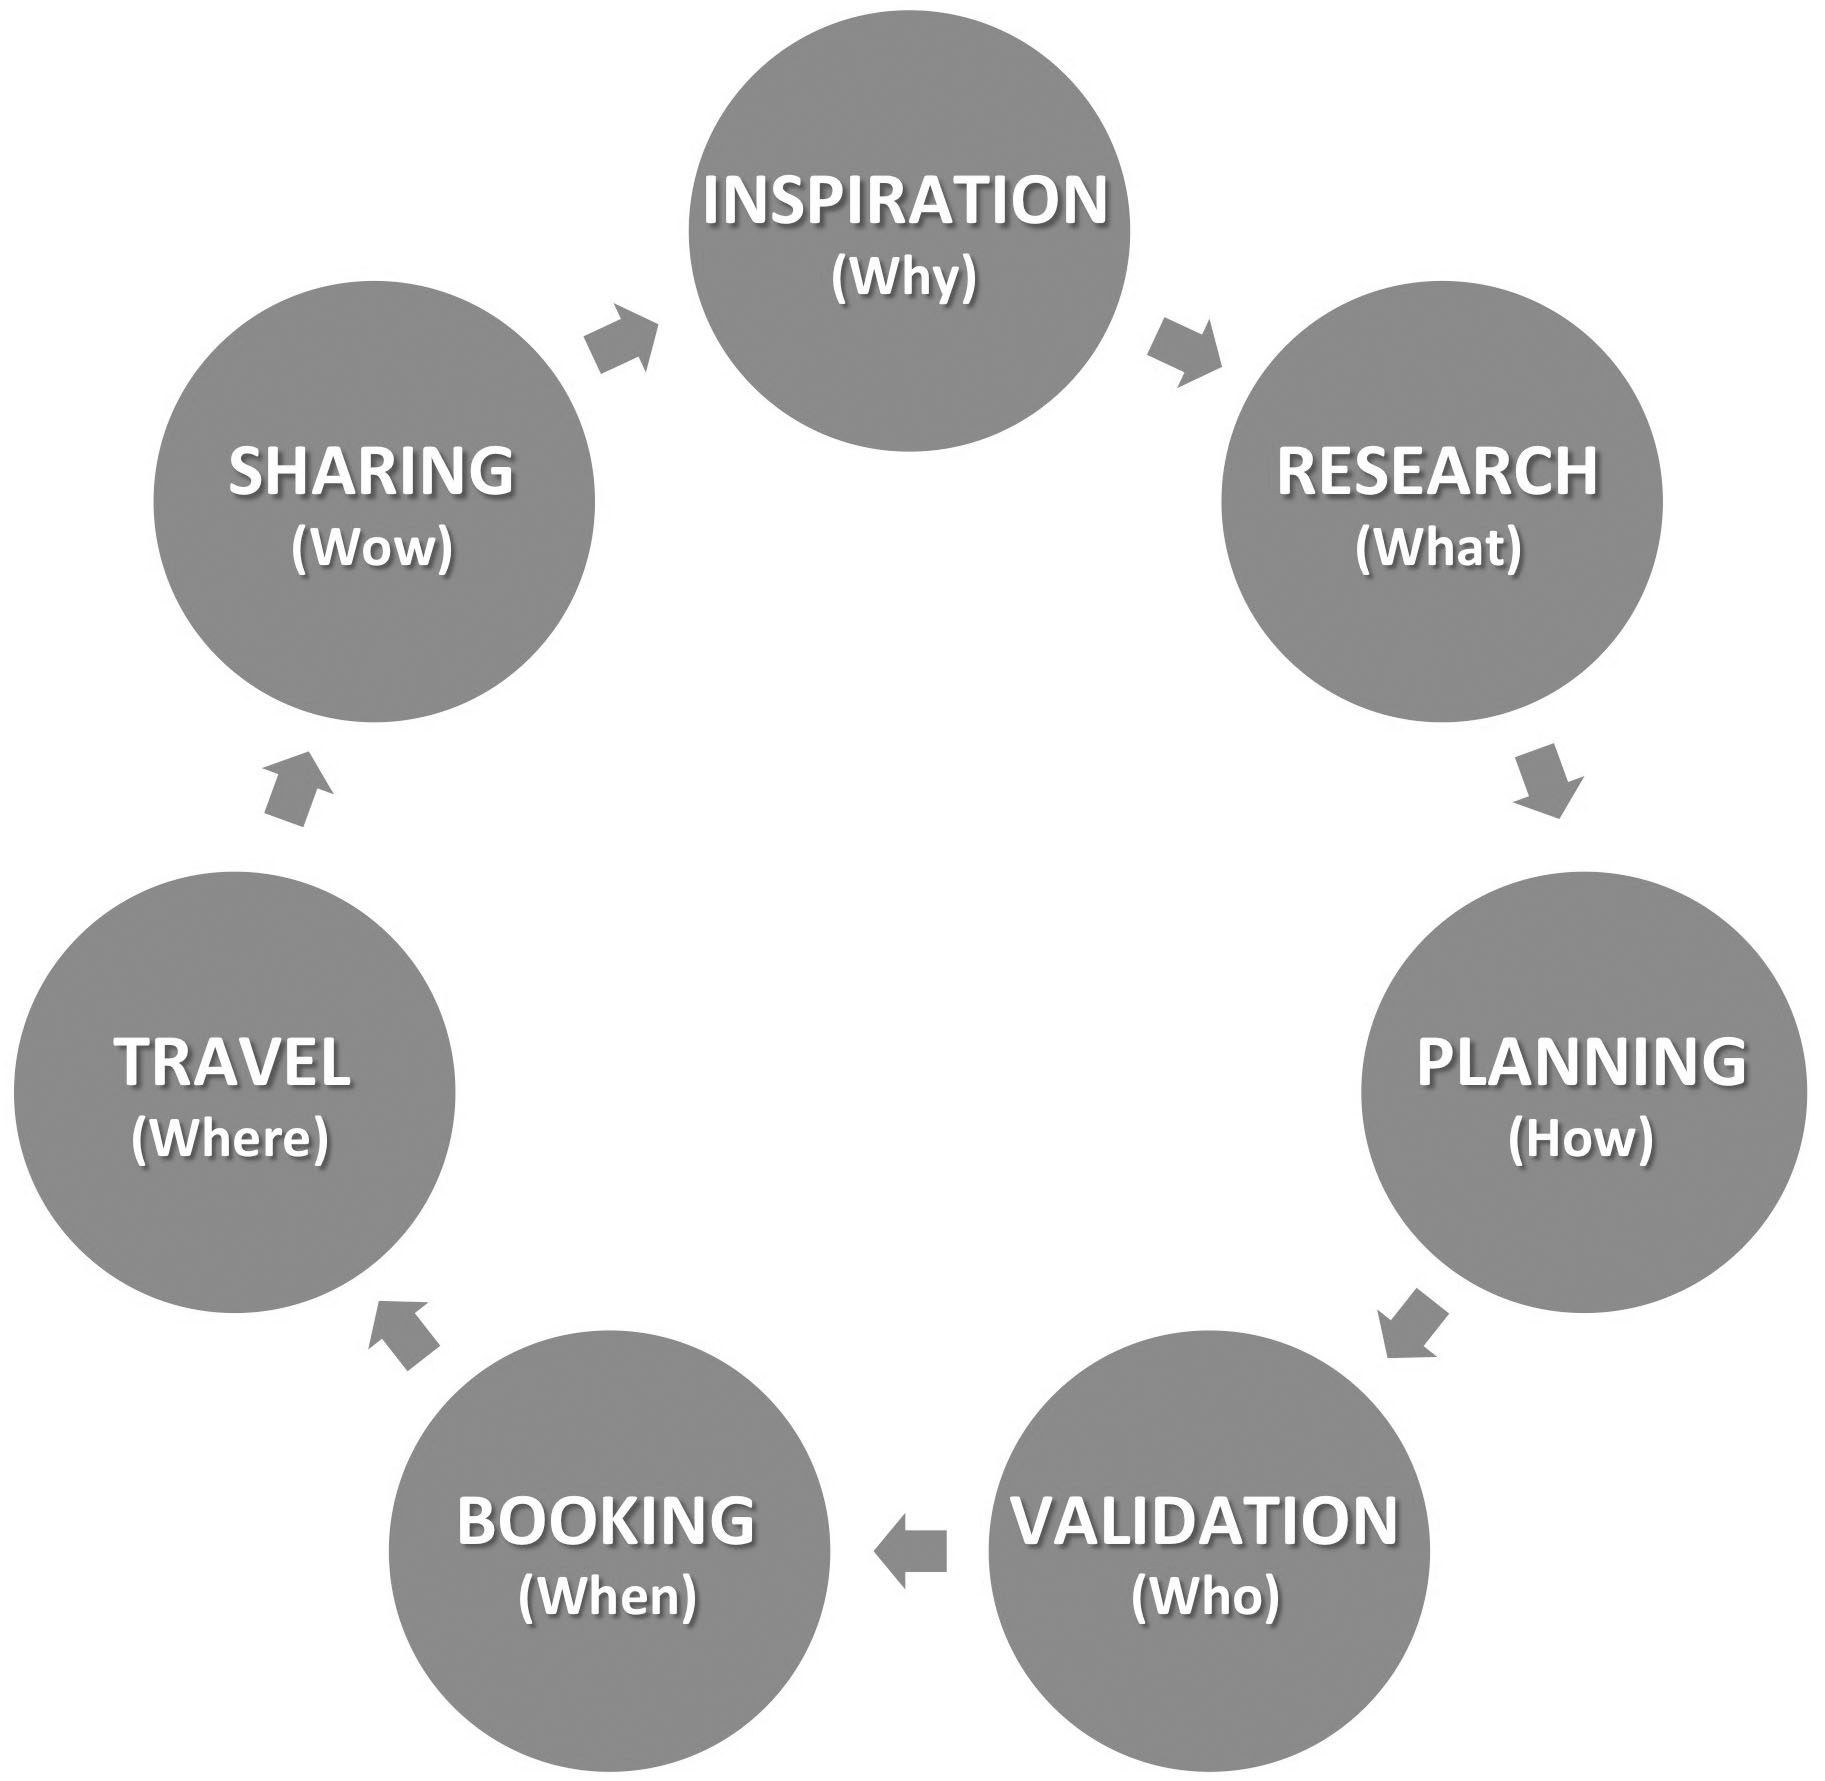
\includegraphics[width=.5\textwidth]{7stages.jpg}
\caption[The Seven Step Travel Process]{The Seven Step Travel Process\protect\footnotemark}
\label{pic:sevenstages}
\end{center}
\end{figure}
\footnotetext{\cite{cole:7step}, Seite 8}

Hierbei ist eine immer stärkere Verschiebung hin zu den digitalen Medien zu beobachten. Inspiration kann durch Urlaubsfotos oder Berichte in Sozialen Netzwerken geschehen. In Foren, Wikis, Onlinemagazinen und Anbieterwebseiten können die für Selektion, Planung und Validierung notwendigen Informationen recherchiert werden. Die Buchung kann über Internetportale oder auf Anbieterwebseiten vorgenommen werden, wobei sowohl der Preis für den Kunden als auch die transaktionsgebundenen Kosten für die Vermittlung hierbei je nach Buchungskanal deutlich schwanken können.\footnote{Bei Buchung über die Webseite eines Hotels fallen z.B. 3\% Gebüren für einen Channelmanager an. Internetportale wie HRS oder Booking.com berechnen zusätzlich 15\% Provision an das Hotel. Quelle: Expertenbefragung} Während des touristischen Erlebnisses selbst kann der Gast sowohl als Konsument als auch als Produzent von Informationen über den Urlaubsort oder den gastronomischen Betrieb in Erscheinung treten. Die Phase Nachbereitung und Weitergabe ist von der Weitergabe von Informationen und Emotionen geprägt.\footnote{vgl. \cite{buhl}}


% subsection customer_journey_im_tourismus (end)



% section tourismus_und_gastgewerbe (end)

\newpage
\section{Technische Möglichkeiten der digitalen Kontaktaufnahme} % (fold)
\label{sec:technologien}

\subsection{QR Codes} % (fold)
\label{sub:qr_codes}
\buzz{QR Codes} (QR für „Quick Response“) sind zweidimensionale Barcodes, die mit Hilfe von Smartphone–Apps gelesen und ausgewertet werden können. Die quadratischen Elemente des Codes sind in einem ebenfalls quadratischen Muster angeordnet. Neben den eigentlichen Nutzdaten sind im Code auch Muster zur Erkennung der Ausrichtung\footnote{Hierdurch ist die Ausrichtung der Kamera beim Lesen irrelevant.} sowie Informationen zur Fehlerkorrektur\footnote{Hierdurch wird die Rekonstruktion der Daten selbst bei erheblicher Beschädigung des Codes noch gelesen werden.} enthalten. Die maximale Speicherkapazität beträgt 2953 Byte bei Fehlerkorrekturstufe L (7\%).\footnote{vgl. \cite{iso18004}, Seite 4f}

QR Codes können auch ohne technisches Verständnis kostenlos erstellt\footnote{z.B. \url{http://www.racoindustries.com/barcodegenerator/2d/qr-code.aspx}} und auf Drucksachen jeglicher Art angebracht werden. Der Kunde startet zum lesen der Informationen die entsprechende App auf seinem Smartphone, richtet die Kamera auf den Code. Während des Scans muss das Telefon für etwa ein bis zwei Sekunden still gehalten werden. Nach Abschluss des Scans werden die dekodierten Daten angezeigt, und entsprechende Aktionen können vom Nutzer aus einem Menü ausgewählt werden.\footnote{Etwa der Aufruf einer URL, das Anlegen eines Adressbucheintrags o.ä.} 

\buzz{Denso Wave Incorporated}, die Entwickler und Markenrechtsinhaber der QR Code Technologie,  verlangen keinerlei Gebühren für die Nutzng von QR Codes. Durch Ausnutzung der Fehlerkorrektur ist es möglich, Logos oder andere Grafiken in QR–Codes zu integrieren. Hierdurch kann zwar die Verknüpfung zur eigenen Marke gestärkt werden, allerdings handelt es sich dann nicht mehr um standardisierte QR–Codes. Somit kann es nicht nur zu Leseproblemen sondern auch zu Lizenzforderungen kommen, die sich Denso Wave ausdrücklich vorbehält.\footnote{vgl. \cite{denso-faq}, Nr. 10}
% subsection qr_codes (end)

\subsection{NFC Tags} % (fold)
\label{sub:nfc_tags}
\buzz{NFC} („Near Field Communication“) bezeichnet eine Technologie zur drahtlosen Übertragung von Daten zwischen elektronischen Geräten. Dies können aktive Geräte\footnote{z.B. Smartphones oder stationäre Schreib–Lesegeräte} oder ein aktives Gerät und eine passive Markierung, üblicherweise englisch als \url{Tag} bezeichnet, sein. Der NFC Tag bezieht seine Energie über seine Antenne vom Schreib–Lesegerät. Die theoretisch maximale Entfernung zwischen Sender und Empfänger beträgt 10cm, in der Praxis sind jedoch wenige Millimeter bis ca. 4cm üblich. Die Datenübertragungsrate beträgt hierbei bei maximal 414 Kilobit pro Sekunde. Außer der räumlichen Nähe ist keinerlei vorherige Konfiguration\footnote{wie z.B. das bei Bluetooth notwendige Pairing} notwendig.\footnote{vgl. \cite{nfcforum:about} sowie \cite{google:nfc}, 2:52 Min.}

NFC Tags sind es in verschiedenen Formen und Größen erhältlich. Üblich sind z.B. die Integration in Schlüsselanhänger oder Scheckkarten, aber auch Aufkleber, die an bzw. hinter beliebigen, dünnen Gegenständen platziert werden können. Die Speicherkapazität beträgt zwischen 96 Bytes (Type~1 Tag) und 32 Kilobytes (Type~4 Tag).\footnote{\cite{nfcforum:spec}, Seite 14} NFC Tags können mithilfe eines Smartphones und kostenlos erhältlichen Anwendungen ohne technisches Verständnis beschrieben werden.

Neben Übertragung von Text oder Dateien ist durch NFC auch der Aufruf von Webseiten, die Übergabe von Konfigurations- oder Verbindungsparametern oder die Veränderung von Einstellungen oder das Ausführen von beliebigen, zuvor definierten Anwendungen auf dem Smartphone möglich.

% subsection nfc_tags (end)

\subsection{Bluetooth} % (fold)
\label{sub:bluetooth}

\buzz{Bluetooth} ist eine Technologie zum Aufbau eines \ac{WPAN}, also eines kabellosen, räumlich eng begrenzten\footnote{i.d.R. 10 Meter, jedoch nicht von der Spezifikation beschränkt, vgl. \cite{bluetooth:smart}} Netzwerks. Hierbei werden durch das sogenannte \buzz{Pairing} Geräte miteinander verbunden, ohne dass hierzu weitere Infrastrukturelemente notwendig wären.\footnote{vgl. \cite{bluetooth:spec}, Seite 1 und Seite 8} Hierbei werden verschiedene Anwendungsfälle und Geräteklassen durch verschiedene \buzz{Profile} unterstützt.  Die Datenübertragungsrate beträgt hierbei bei maximal 24 Megabit pro Sekunde.\footnote{vgl. \cite{bluetooth:sigv1}, Seite 17f sowie \cite{bluetooth:sigv3}, Seite 277}

Auch wenn komplexere Fälle möglich sind, bestehen typische Bluetooth–Verbindungen beim Endverbraucher zwischen zwei Geräten, meist einem Sender und einem Empfänger. Beispiele hierfür ist der Anschluss von Tastatur und Maus an ein Notebook oder das Abspielen von Musik auf Bluetooth–Lautsprechern. Auch die Übertragung von elektronischen Visitenkarten oder anderen Dateien ist möglich. Die Verbindung wird hierbei auf Ebene des Betriebssystems \acused{OS} (\ac{OS} für engl. Operating System) zwischen den Geräten hergestellt, das Senden wird i.d.R. durch die Auswahl eines entsprechenden Menüpunktes in der jeweiligen Anwendung initiiert. Der Empfänger entscheidet dann per Dialogfenster, ob er die Daten empfangen möchte.

Aufgrund der Vielzahl von Übertragungsprofilen, von denen jedes Gerät nur eine Teilmenge unterstützt kann nicht davon ausgegangen werden, dass jedes Bluetooth–Gerät mit jedem anderen auf die gewünschte Art kommunizieren kann, selbst wenn das Pairing erfolgreich ist.\footnote{vgl. \cite{bluetooth:spec}, Seite 7}
% subsection bluetooth (end)

\subsection{Bluetooth Low Energy} % (fold)
\label{sub:bluetooth_low_energy}

Das in der Bluetooth Spezifikation 4.0 eingeführte Low Energy Profil (BLE\acused{BLE}) ermöglicht Geräte mit extrem niedrigem Stromverbrauch. Hierdurch sind Anwendungen möglich, welche wie bei der Nutzung von passiven Elementen unabhängig von weiterer Infrastruktur sind, und trotzdem von den Möglichkeiten aktiver Sendern\footnote{z.B. das Senden von Analysedaten oder Messung des Abstands zwischen Sender und Empfänger} profitieren können.\footnote{vgl. \cite{bluetooth:smart}}

BLE Geräte sind auch unter den Markenbezeichnungen \buzz{iBeacon} erhältlich. 
% subsection bluetooth_low_energy (end)

\subsection{Lesbare Internetadressen} % (fold)
\label{sub:kurzlinks}
Die am wenigsten technische Möglichkeit, Kunden auf das digitale Angebot eines Unternehmens hinzuweisen ist die Angabe einer menschenlesbaren\footnote{Lesbar schließt für diese Zwecke auch Piktogramme von bekannten Internetdiensten ein.} \ac{URL}, also Internetadresse\footnote{Obwohl der Begriff URL eine Internetadresse in sehr allgemeiner Form beschreibt, wird er in dieser Arbeit der Lesbarkeit halber synonym zu „WWW–Adresse“ verwendet.} auf Drucksachen. Diese werden vom Kunden in das Smartphone oder in den Webbrowser seines Computers von Hand eingegeben. Je länger diese URL ist, desto schwieriger ist dies.

Daher ist ab einer gewissen Länge bzw. Komplexität der Adresse eine Methode notwendig, mit der diese kürzer bzw. einfacher zu machen. Zur Erstellung solcher Kurz–URLs stehen kostenlose Internet–Dienste\footnote{z.B. Goo.gl, Ow.ly, FixURL.de oder Bit.ly} sowie Funktionen des \ac{CMS}\footnote{Hier werden kurze, freundliche Adressen wie z.B. \url{http://DieKrone.de/feedback} zur eigentlichen Seite \url{https://secure.holidaycheck.de/hotelbewertung_abgeben.php?action=hotelselect&entityId=161279} weitergeleitet.} zur Verfügung. 
% subsection kurzlinks (end)

\subsection{Nachrichtendienste und Chatsysteme} % (fold)
\label{sub:internet_nachrichtendienste}
Kurznachrichtendienste und Chatsysteme wie z.B. Whatsapp, SMS, Twitter, Facebook–Messenger, iMessage oder Skype können zur digitalen Kommunikation mit Kunden genutzt werden. Die Kommunikationspartner werden hierbei entweder durch Benutzernamen identifiziert, wodurch jedes internetfähige Gerät genutzt werden kann, oder die Kommunikation wird über die Mobilfunknummer der Beteiligen vermittelt, was die Nutzung eines Smartphones notwendig macht, selbst wenn die eigentliche Datenübertragung während der Verbindung über das Internet abgewickelt wird.

Sowohl Twitter als auch Facebook können hierbei nicht nur zur privaten, sondern auch zur öffentlichen Kommunikation genutzt werden.

Aufgrund der hohen Anforderung bzgl. synchroner Kommunikation ist diese Möglichkeit nicht optimal für kleine Betriebe. Die eigentliche Kontaktaufnahme muss zudem über eine der anderen Methoden geschehen. Daher werden Nachrichtendienste und Chatsysteme hier nur der Vollständigkeit erwähnt.
% subsection internet_nachrichtendienste (end)

\subsection{Hotel--Apps} % (fold)
\label{sub:hotel_apps}
Speziell auf das Hotel oder auf das \ac{PMS} zugeschnittene Smartphone–Apps\footnote{z.B. Protel Voyager} ermöglichen durch den Zugriff auf die Daten des Reservierungssystems eine hohe Integrationsstufe und zielgerichtete Kommunikation. Auch sind Funktionen wie die Abfrage von Reservierungs– oder Rechnungsdaten oder Bestellungen beim Zimmerservice möglich.

Die eigentliche Kontaktaufnahme muss zudem über eine der anderen Methoden geschehen, damit der Gast die Anwendung installiert. Des  weiteren richtet sich das Angebot nur an tatsächliche Gäste, nicht wie die anderen hier vorgestellten Technologien auch an Interessenten. Daher werden Hotel–Apps hier nur der Vollständigkeit erwähnt.

% subsection hotel_apps (end)

% section technologische_moglichkeiten_der_digitalen_kontaktaufnahme (end)


\newpage
\section{Bewertungskriterien} % (fold)
\label{sec:kriterien}

\subsection{Betrachtung von Seiten des Betriebs} % (fold)
\label{sub:anforderungen_auf_seiten_des_betriebs}
Es werden die möglichen Einsatzorte sowie die möglichen Einsatzzwecke wie in den Kapiteln~\myref{sec:einsatzorte} und \myref{sec:einsatzzwecke} beschrieben bewertet. Ebenso wird untersucht, ob die jeweilige Technologie für die Ausbringung in großen Mengen, etwa auf Visitenkarten geeignet ist oder nicht.

Des weiteren werden die Hardwareanforderungen und die anfallenden Kosten, sowohl für die Erstellung als auch für den laufenden Betrieb, ermittelt. 
% subsection anforderungen_auf_seiten_des_betriebs (end)

\subsection{Betrachtung von Seiten des Kunden} % (fold)
\label{sub:anforderungen_auf_seiten_des_kunden}
Von Kundenseite wird die benötigte Hard– und Software, der Bekanntheits– und Verbreitungsgrad sowie die Benutzerfreundlichkeit der jeweiligen Technologie betrachtet. 
% subsection anforderungen_auf_seiten_des_kunden (end)

\subsection{Sicherheit} % (fold)
\label{sub:sicherheit}
Bei der digitalen Kontaktaufnahme steht „Spoofing“ als Angriffsart im Vordergrund. Darunter versteht man die Ausbringung von gefälschten Kontaktmedien, die den Kunden mit falschen Informationen versorgt. Des weiteren kann der Kunde auf gefälschte Webseiten geführt werden, auf denen Kundeninformationen in den Besitz des Angreifers gelangen können.\footnote{vgl. \cite{gilchrist}, Abschnitt 9.1} Ein solcher Angriff hat somit Ähnlichkeit mit Phishing.\footnote{engl. Kunstwort aus „Password“ und „Fishing”, vgl. \cite{bsi:phishing}}

Falls auf Seiten des Betriebs aktive Geräte zum Einsatz kommen, kann ein Angreifer durch Hacking, also dem gezielten Einsatz von speziell gestalteten Daten diese manipulieren, für andere Zwecke zu nutzen oder ganz außer Betrieb setzten.\footnote{vgl. \cite{gilchrist}, Abschnitt 9.2} 
% subsection sicherheit (end)
% section bewertungskriterien (end)


%!TEX root = /Users/stwaidele/Dropbox (Leisinger)/02 - AKAD/Projektbericht/Möglichkeiten der Digitalen Kontaktaufnahme im Endkundenbereich/vorlage.tex

\section{Einsatzorte} % (fold)
\label{sec:einsatzorte}

\subsection{Quellmedien} % (fold)
\label{sub:quellmedien}
Rein technisch betrachtet ist das Quellmedium beim Untersuchten Meidenbruch bin zur digitalen Kommunikation meist ein Druckerzeugnis. Dies kann der Briefbogen, das Hausprospekt, eine Broschüre, ein Schild, Plakat oder die Visitenkarte sein. Das Wechselmedium ist entweder direkt darauf gedruckt, oder im Falle von elektronischen Varianten hinter einem entsprechenden Logo oder Hinweistext platziert. Möglich wären zwar auch Werbespots. In der klassischen Form des Werbespots sind diese für die betrachtete  Unternehmensgröße jedoch zu teuer.

% subsection quellmedien (end)

\subsection{An Stationen des Customer Journey} % (fold)
\label{sub:stationen_des_customer_journey}
Es sind diejenigen Phasen der Customer Journey bei denen der Gast direkten Kontakt hat, während denen gastronomische Betriebe die digitale Kontaktaufnahme beeinflussen können. Dies beginnt bei der Buchung, ist in der Erlebnisphase am ausgeprägtesten und reicht bis zur Nachbereitung.

Während des Aufenthalts können entsprechende Hinweise auf Drucksachen und Schildern platziert werden um den Gast auf die digitalen Angebote des Betriebs zu führen. Dies kann an jedem \ac{POI}, also an Sehenswürdigkeiten jeglicher Art wie zum Beispiel an einem Gemälde, am Speisekartenaushang, an der Eingangstür oder im Rosengarten sein.

Bei Buchung und Nachbereitung sind diese Hinweise in der Korrespondenz zu platzieren.\footnote{Im Falle von E–Mails wird somit ein Wechsel von persönlicher zu unpersönilicher elektronischer Kommunikation angestrebt.}
% subsection stationen_des_customer_journey (end)

\subsection{In der Gastronomie} % (fold)
\label{sub:gastronomie}
In gastronomischen Betrieben lässt sich der Aufenthalt bzw. die Erlebnisphase der Customer Journey vereinfacht in fünf Phasen einteilen: Vor dem Besuch, vor der Bestellung, nach der Bestellung, während des Verzehrs\footnote{Bei mehrgängigen Menüs durch wartezeiten auf den nächsten Gang unterbrochen} und nach dem Besuch. Die Phasen eignen sich unterschiedlich gut für die digitale Kontaktaufnahme.  Vor der Bestellung und während des Verzehrs sind Verzögerungen durch den Gebrauch von Smartphones nicht wünschenswert.\footnote{Auch wenn die Behauptungen, dass der Service in einem New Yorker Restaurant sich durch Smartphonenutzung um durchschnittlich 50 Minuten verzögert wird (vgl. \cite{craiglist:slow}) nicht belegt sind, sind die geschilderten Phänomene zumindest mit kürzeren Zeitangaben doch plausibel. (vgl. \cite{craiglist:fake})} Vor dem Besuch, nach der Bestellung sowie nach den Besuch entstehen hierdurch keine Probleme, sondern für Gast und Betrieb vorteilhafte Anwendungsfälle. 

Der Gast kann durch entsprechende Hinweise am Speisekartenaushang, im Eingangsbereich, auf der Speisekarte, auf Tischaufstellern oder auf der Rechnung zu den digitalen Angeboten des Betriebs geleitet werden.
% subsection gastronomie (end)

\subsection{In der Hotellerie} % (fold)
\label{sub:hotellerie}
In Beherbergungsbetrieben hält sich der Gast während des Aufenthalts zwischen Anreise (Check–In) und Abreise (Check–Out) an unterschiedlichen Orten innerhalb des Betriebs auf. Für die Einnahme der Mahlzeiten gilt das im Abschnit~\myref{sub:gastronomie} gesagte. Weitere mögliche Orte der digitalen Kontktaufnahme sind das Zimmer des Gastes, öffentliche Bereiche wie Flure, Aufenthaltsräume und der Wellnessbereich. Des weiteren können solche Angebote besonders an Orten, an denen viele Gäste warten, gerne angenommen werden. Beispiele hierfür sind im Bereich der Aufzüge oder in der Lobby.

% subsection hotellerie (end)


% section einsatzorte (end)

\addtocontents{toc}{\protect\newpage}
\section{Einsatzzwecke} % (fold)
\label{sec:einsatzzwecke}

\subsection{Zielmedien} % (fold)
\label{sub:zielmedien}
Die Zielmedien können technisch in direkt und indirekt erreichte Ziele unterteilt werden. Bei direkter Zielerreichung wird die vom Gast erwartete Information direkt durch das Wechselmedium übertragen. Hierbei ist die Größe der Information durch die Speicherkapazität der verwendeten technischen Lösung begrenzt. Diese Methode funktioniert ohne Internetzugriff.  Im Gegensatz dazu wird bei der indirekten Zielerreichung lediglich eine \ac{URL} zur Information übergeben. Hierbei ist die Datenmenge lediglich durch die Bandbreite bzw. durch die Geduld des Kundens begrenzt.
% subsection zielmedien (end)

\subsection{Beeinflussung Customer Journey} % (fold)
\label{sub:beeinflussung_customer_journey}
Touristische Betriebe können durch Lenkung der digitalen Aktivitäten der Kunden auf Customer Journey weiterer Interessenten einwirken. Wenn zufriedene Gäste ihre Erlebnisse und Bewertungen anderen mitteilen, dann hat dies positive Auswirkungen auf deren Phasen der Inspiration, Recherche und Planung. Somit bieten sich generelle Hinweise auf Social Media Dienste an, um das Teilen der Urlaubserlebnisse zu fördern. 

\begin{figure}[H]
\begin{center}

\includegraphics[width=.8\textwidth]{zielcj.jpg}
\caption[Beispiel: Hinweis auf Social Media Dienste]{Beispiel: Hinweis auf Social Media Dienste\protect\footnotemark}
\label{pic:zielcj}
\end{center}
\end{figure}
\footnotetext{Rückseite der Visitenkarte eines Hotels}

Des weiteren können Gäste gezielt auf Webseiten oder Social Media Angebote des Betriebs gelenkt werden. Hier kann der Kunde dann mit Informationen versorgt werden. Wenn der Kunde dazu animiert werden kann, die digitalen Angebote des Betriebs selbst in den Netzwerken zu teilen, werden dadurch diese im Einfluss gestärkt.\footnote{vgl. \cite{fb:news}}
% subsection beeinflussung_customer_journey (end)

\subsection{Kunden mit Information versorgen} % (fold)
\label{sub:kunde_mit_information_versorgen}
Bei ausreichender Speicherkapazität des Wechselmediums kann der Kunde direkt mit Informationen versorgt werden. Hierfür bieten sich Kontaktinformationen\footnote{Als VCard formatierte Informationen lassen sich direkt in das Adressbuch von Smartphones importieren.}, Terminkalendereinträge oder erklärende Texte\footnote{z.B. zu Bildern, oder Öffnungszeiten} an.

Während reine Informationstexte keinen oder nur sehr geringen Mehrwert gegenüber den gedruckten Informationen bieten, sind entsprechend formatierte Kontakt– oder Termininformationen für Kunden und Unternehmen nützlich, da durch sie die manuelle Eingabe in das Smartphone vermieden werden kann und somit diese Informationen wahrscheinlicher beim Kunden gespeichert werden.

Bei indirekten Zielen kann der Kunde auf Webseiten beliebiger Art geführt werden. Das Wechselmedium übergibt dazu die entsprechende \ac{URL}, die mit dem Webbrowser des Smartphones aufgerufen werden kann. Hierbei sollte es sich um eine für Mobilgeräte optimierte Seite handeln.

Mögliche Zielseiten können die Unternehmenswebsite, der Firmeneintrag bei Bewertungsdiensten, das Profil des Betriebs bei Social Media Diensten, Gewinnspiele, eine Eintragung für den Newsletter oder auch die Downloadadresse der Betriebseigenen App sein. Somit können die entsprechenden Angebote beworben bzw. entsprechende Aktivitäten gefördert werden.

% subsection kunde_mit_information_versorgen (end)

\subsection{Informationen von Kunden erhalten} % (fold)
\label{sub:informationen_vom_kunden_erhalten}
Durch den Einsatz von aktiven Elementen bzw. indirekten Zielen kann auch das Unternehmen Daten über seine Kunden sammeln. Dies kann in anonymer Form über die Zugriffsdaten der referenzierten Webseiten oder falls dies die eingesetzte Technologie dies ermöglicht einen Zugriffszähler im Wechselmedium\footnote{z.B. in Bluetooth Low Energy Geräten}. Durch mehrere Elemente kann auch der Pfad von Kunden erfasst oder geschätzt werden. Über die HTML5 Geolocation \ac{API} ließe sich sogar die exakte Position des Kunden beim Seitenabruf ermitteln.\footnote{z.B. \url{http://www.torbenleuschner.de/files/geo.htm}}

Durch entsprechende Gestaltung der referenzierten Webseite können auch personalisierte Daten erfasst werden. Hierzu ist z.B. ein Newsletterangebot, die Abfrage von Kundenfeedback oder ein Gewinnspiel geeignet. Hierbei sind jedoch unbedingt die Vorschriften des Datenschutzgesetzes zu beachten.
% subsection informationen_vom_kunden_erhalten (end)

% section einsatzzwecke (end)

\section{Bewertung der Technologien} % (fold)
\label{sec:bewertung}

\subsection{Bewertung QR Codes} % (fold)
\label{sub:bewertung_qr_codes}
QR Codes können für alle Quellmedien und für alle Zielmedien eingesetzt werden. Der zur Erstellung von Drucksachen ohnehin notwendige Workflow wird lediglich um die Erstellung des Codes erweitert, was mit Hilfe von kostenlosen Webdiensten ohne großen Aufwand möglich ist.\footnote{z.B. \url{http://www.racoindustries.com/barcodegenerator/2d/qr-code.aspx}} Die Kosten für identische QR–Codes beschränken sich somit lediglich auf ebendiese Erstellung und bleiben unabhängig von der Ausbringungsmenge konstant. Es entstehen keine Variablen Kosten. Im Betrieb treten keine laufenden Kosten auf.

QR Codes sind mit allen gängigen Smartphones und Tablet–PCs lesbar, allerdings i.d.R. nicht mit vorinstallierter Software. Der Kunde muss somit einmalig vor der ersten Nutzung eine entsprechende Lese–App herunterladen und installieren. Vor jedem Lesen, muss diese aktiviert werden und mit der Kamera der QR Code erfasst werden. Hierbei kann es je nach Größe des gedruckten Codes, der Informationsdichte und den Lichtverhältnissen zu Fokusproblemen kommen, die das Lesen erschweren.   

Die maximale Speicherkapazität ist somit nur theoretisch erreichbar. Je größer die zu speichernde Datenmenge, desto feiner werden bei gleich bleibender Abbildungsgröße die zu scannenden Strukturen. Die Abbildungsgröße ist jedoch aufgrund der Nutzung der Smartphone–Kamera limitiert.\footnote{Auch bei extrem groß dargestellten QR–Codes muss dieser durch Anpassung des Abstandes so verkleinert werden, dass er ganz von der Kamera erfasst wird.} So war keines der getesteten Smartphones\footnote{Apple iPhone 5 sowie Samsung Galaxy S5 mini} in der Lage, einen V40 QR–Code zu erkennen. Auch bei kleineren Datenmengen treten bereits deutliche Unterschiede in der Erkennungsleistung sowohl zwischen den Geräten als auch zwischen den verwendeten Apps auf. Für die Übertragung einer \ac{URL}, Kontaktinformationen oder kurze erklärende Texte ist jedoch zuverlässig möglich.

Von den 174 Teilnehmenden der Umfrage gaben lediglich 26 an, QR Codes nicht zu kennen und weitere 28, sich nicht für QR Codes zu interessieren. Der Bekanntheitsgrad von QR Codes liegt somit bei knapp 60\% (120 Personen). Von den 119 gegebenen Angaben zur Benutzerfreundlichkeit waren 93 bzw. 78\% im Bereich „Gut“ oder besser.

Von den 112 Teilnehmenden, die QR Codes nutzen, nutzen 30 (27\%) NFC Tags, 99 (88\%) Bluetooth, 12 (11\%) \ac{BLE} und 80 (71\%) Kurzlinks. Von diesen Personen bewerteten die  Benutzerfreundlichkeit von NFC Tags 22 (20\%), von Bluetooth 72 (64\%), von \ac{BLE} 4 (4\%), und von Kurzlinks 65 (58\%) im Vergleich zu QR Codes als gleich oder besser.

Beim Einsatz von QR Codes besteht die Möglichkeit Spoofings durch unbemerktes Überkleben mit Codes, die falsche Informationen beinhalten oder dazu führen. Diese Vorgehensweise ist besonders bei einzeln platzierten QR Codes möglich. 
% subsection bewertung_qr_codes (end)

\subsection{Bewertung NFC Tags} % (fold)
\label{sub:bewertung_nfc_tags}
NFC Tags können mit Einschränkungen für alle Quellmedien und für alle Zielmedien eingesetzt werden. Der mit einem NFC-fähigen Smartphone oder Tablet–PC beschriebene NFC Tag ist das Kontaktmedium oder wird hinter dem Medium angebracht. Durch den Preis von einigen Cent pro NFC–Aufkleber\footnote{Januar 2015: 0,35€ pro Aufkleber bei NFC-Tag-Shop.de} sowie der Notwendigkeit jeden NFC Tag einzelnen zu beschreiben entstehen bei der Ausbringung identischer Kopien auf Massenartikeln jedoch variable Kosten. Hierdurch werden die möglichen Quellmedien durch die Wirtschaftlichkeit begrenzt. Im Betrieb treten keine laufenden Kosten auf.

Es ist nicht möglich, NFC Tags mit Apple Smartphones oder Tablet–PCs zu lesen. In der aktuellen Modellgeneration ist zwar ein NFC Lesechip eingebaut, dieser ist jedoch nicht allgemein einsetzbar, sondern der Apple–eigenen Bezahlsoftware vorbehalten.\footnote{vgl. \cite{zdnet:applenfc}}
Somit sind mindestens 12,7\% der neu verkauften Smartphones nicht in der Lage, Informationen aus NFC Tags auszulesen.\footnote{\cite{garnter:os}, Tabelle 2}

Von den 174 Teilnehmenden der Umfrage gaben 72 an, NFC Tags nicht zu kennen und weitere 38, sich nicht für NFC Tags zu interessieren. Der Bekanntheitsgrad von NFC Tags liegt somit bei knapp 37\% (64 Personen). Von den 45 gegebenen Angaben zur Benutzerfreundlichkeit waren 28 bzw. 62\% im Bereich „Gut“ oder besser. 

Von den 32 Teilnehmenden, die NFC Tags nutzen, nutzen 30 (94\%) QR Codes, 30 (94\%) Bluetooth, 8 (25\%) \ac{BLE} und 26 (81\%) Kurzlinks. Von diesen Personen bewerteten die  Benutzerfreundlichkeit von QR Codes 19 (59\%), von Bluetooth 23 (72\%), von \ac{BLE} 3 (9\%), und von Kurzlinks 19 (59\%) im Vergleich zu NFC Tags als gleich oder besser.

Um Missbrauch zu verhindern, können NFC Tags beim Beschreiben mit einem Schreibschutz versehen werden. Dieser schließt dann aber auch spätere gewollte Änderungen an den gespeicherten Daten aus, so dass zur Aktualisierung ein neuer NFC Tag verwendet werden muss. Spoofing ist somit lediglich durch das Anbringen von weiteren NFC Tags möglich.
% subsection bewertung_nfc_tags (end)

\subsection{Bewertung Bluetooth} % (fold)
\label{sub:bewertung_bluetooth}
Um Bluetooth als Kontaktmedium zu nutzen, wird eine Sendestation benötigt, die mit dem Gerät des Kunden\footnote{Neben einem Smartphone kommen hier auch Tablet–PCs oder Notebooks mit Bluetooth–Schnittstelle in Frage} Kontakt aufnimmt und die gewünschten Daten überträgt. Die Hardwareanforderungen hierzu sind niedrig, so dass ein entsprechend programmiertes Smartphone oder ein Einplatinencomputer\footnote{z.B. Raspberry Pi oder Arduino} ausreicht. Die Sendestation kann aufgrund der Reichweite auch in einigen Metern Entfernung zur Position des Kunden platziert werden. Aufgrund dieser notwendigen Infrastruktur ist Bluetooth nicht für die Ausbringung auf Massenartikeln geeignet. Die einmaligen Kosten belaufen sich auf den Programmieraufwand für die gewünschte Funktionalität. Pro Sendestation entstehen zusätzlich variable Kosten, die von der eingesetzten Hardware abhängig sind.\footnote{z.Zt. kostet ein Raspberry Pi ca. 40€ bei \url{Amazon.de}} Während des Betriebs fallen Stromkosten an.

Alle gängigen Smartphones, Tablet–PCs und viele Notebooks können über Bluetooth mit der Sendestation Daten austauschen. Hierzu ist allerdings ein Kopplungsvorgang notwendig, der einige Sekunden dauert und die aktive Mitwirkung des Kundens erfordert\footnote{Bluetooth ggf. aktivieren, Umgebung nach Geräten durchsuchen, Verbindung bestätigen.} Anschließend ist die Übertragung von Daten entsprechend der von beiden Geräten unterstützten Protokolle möglich. Die Schnittmenge der von Sender und Empfänger unterstützen Übertragungsprotokolle beschränkt die möglichen Kontaktmöglichkeiten. So unterstützen Apple–Geräte weder die Übertragung von Texten und Bildern noch von Kontaktinformationen. Bei anderen Herstellern kann die entsprechende Unterstützung dieser Funktionalität von Gerät und Betriebssystemversion abhängig sein.

Von den 174 Teilnehmenden der Umfrage gaben 7 an Bluetooth nicht zu kennen und weitere 22, sich nicht für Bluetooth zu interessieren. Der Bekanntheitsgrad von Bluetooth liegt somit bei über 83\%. Von den 151 gegebenen Angaben zur Benutzerfreundlichkeit waren 120 bzw. 79\% im Bereich „Gut“ oder besser.

Von den 140 Teilnehmenden, die Bluetooth nutzen, nutzen 99 (71\%) QR Codes, 30 (21\%) NFC Tags, 13 (9\%) \ac{BLE} und 95 (68\%) Kurzlinks. Von diesen Personen bewerteten die  Benutzerfreundlichkeit von QR Codes 64 (46\%), von NFC Tags 22 (16\%), von \ac{BLE} 2 (1\%), und von Kurzlinks 73 (52\%) im Vergleich zu Bluetooth als gleich oder besser.

Missbrauch ist wegen der Reichweite von Bluetooth durch von Angreifern platzierten Sendern auch aus einigen Metern Entfernung möglich, aufgrund der benötigen Stromversorgung jedoch aufwändig. Mögliche temporäre und mobile Spoofing–Angriffe mit Smartphones, die sich als betriebseigene Sender ausgeben sind möglich und nur schwer zu bemerken. 

% subsection bewertung_bluetooth (end)

\subsection{Bewertung Bluetooth Low Energie} % (fold)
\label{sub:bewertung_bluetooth_low_energie}
Für den Einsatz von \ac{BLE} Sendern zur Kontaktaufnahme gilt aufgrund der gemeinsamen Basistechnologie zunächst das für Bluetooth gesagte. Die Sender sind jedoch fertig konfiguriert im Handel erhältlich, was den Einrichtungsaufwand reduziert. Außerdem entfällt die Notwendigkeit der Kopplung mit dem Empfänger. \ac{BLE} benötigt auf Kundenseite Bluetooth 4.0 fähige Endgeräte, welche aber bereits seit 2011 im Handel sind und eine große Menge der aktuellen und vorhergehenden Generation von Smartphones einschließt.\footnote{\cite{gilchrist}, Abschnitt 1.4}

Bei den vom Sender übertragenen Daten handelt es sich lediglich um eine weltweit eindeutige Identifikation, sowie der Entfernung zwischen Sender und Empfänger. Eine Übersetzung in für den Kunden nützliche Daten erfolgt dann in einer betriebsspezifischen Smartphone–App\footnote{Die Nutzung von betriebsspezifischen Apps wird in dieser Arbeit nicht untersucht.} oder in Form von Passbook Codes.\footnote{Dies stellt einen Spezialfall der Weitergabe von Informationen an Kunden dar.} Die Kosten pro BLE Sender betragen je nach Hersteller zwischen 8€ und 40€. Passbook Codes können zu geringen Kosten bei Internetdiensten erstellt werden.\footnote{z.B. \url{http://www.passcreator.de/preise/}} Aufgrund der technischen Voraussetzungen ist \ac{BLE} nicht für die mehrfache Ausbringung identischer Exemplare, sondern nur für an einen bestimmten Ort gebundene Quellmedien geeignet. 

Von den 174 Teilnehmenden der Umfrage gaben 117 an \ac{BLE} nicht zu kennen und weitere 28, sich nicht für \ac{BLE} zu interessieren. Der Bekanntheitsgrad von \ac{BLE} liegt somit bei 17\%. Von den 15 gegebenen Angaben zur Benutzerfreundlichkeit waren 6 bzw. 40\% im Bereich „Gut“ oder besser.

Von den 13 Teilnehmenden, die \ac{BLE} nutzen, nutzen 12 (92\%) QR Codes, 8 (62\%) NFC Tags, 13 (100\%) Bluetooth und 12 (92\%) Kurzlinks. Von diesen Personen bewerteten die  Benutzerfreundlichkeit von QR Codes 7 (54\%), von NFC Tags 6 (46\%), von Bluetooth 8 (62\%), und von Kurzlinks 8 (62\%) im Vergleich zu \ac{BLE} als gleich oder besser.

Missbrauch ist wie auch bei Bluetooth durch vom Angreifer platzierte Sender möglich, aufgrund der Unabhängigkeit von externen Stromquellen sogar noch einfacher. Gleiches gilt für temporäre bzw. mobile Angriffe. Neben dem Spoofing ist jedoch auch das Hacking bei BLE Sendern möglich.\footnote{vgl. \cite{gilchrist}, Abschnitt 9.2} 
% subsection bewertung_bluetooth_low_energie (end)

\subsection{Bewertung Kurzlinks} % (fold)
\label{sub:bewertung_kurzlinks}
Kurzlinks können für alle Quellmedien und mit für alle Zielmedien eingesetzt werden. Der zur Erstellung von Drucksachen ohnehin notwendige Workflow wird lediglich um die Erstellung des Links erweitert, was in \ac{CMS} ohne großen Aufwand möglich ist. Die Kosten beschränken sich somit lediglich auf ebendiese Erstellung bleiben unabhängig von der Ausbringungsmenge konstant. Es entstehen keine Variablen Kosten. Im Betrieb treten keine laufenden Kosten auf.

Kurzlinks werden vom Kunden in die Adresszeile des Webbrowsers des Smartphone, Tablet–PC oder Notebook eingegeben. Somit sind sie mit allen Geräten mit vorinstallierter Software nutzbar. 

Von den 174 Teilnehmenden der Umfrage gaben 35 an, Kurzlinks nicht zu kennen und weitere 28, sich nicht für Kurzlinks zu interessieren. Der Bekanntheitsgrad von Kurzlinks liegt somit bei über 63\%. Von den 114 gegebenen Angaben zur Benutzerfreundlichkeit waren 98 bzw. 86\% im Bereich „Gut“ oder besser. 

Von den 104 Teilnehmenden, die Kurzlinks nutzen, nutzen 80 (77\%) QR Codes, 26 (25\%) NFC Tags, 95 (91\%) Bluetooth und 12 (12\%) \ac{BLE}. Von diesen Personen bewerteten die  Benutzerfreundlichkeit von QR Codes 44 (42\%), von NFC Tags 15 (14\%), von Bluetooth 69 (66\%), und von \ac{BLE} 98 (94\%) im Vergleich zu Kurzlinks als gleich oder besser.

Beim Einsatz von Kurzlinks besteht die Möglichkeit des Spoofings durch unbemerktes Überkleben mit \ac{URL}s, die zu falschen Informationen führen. Des weiteren besteht die Möglichkeit, ähnliche Domainnamen, sogenannte „Tippfehler Domains“, zu registriern um die Kunden auf die Webseiten des Angreifers zu lenken.\footnote{vgl. BGH: Urteil vom 22. Januar 2014 - I ZR 164/12 - wetteronline.de}
% subsection bewertung_kurzlinks (end)

\subsection{Zusammenfassung der Bewertungen} % (fold)
\label{sub:zusammenfassung_der_bewertungen}

Die in den vorangegangenen Abschnitten beschriebenen Eigenschaften sind hier nochmals als Tabelle zusammengefasst:

\begin{table}[H]
\begin{center}
\begin{footnotesize}
\begin{tabular}{| l | C{1cm} | C{1cm} | C{1cm} | C{1cm} | C{1cm} |}  \hline                       
  \textbf{Kriterium} & 
	\begin{turn}{90}\textbf{QR Codes\vspace{0.1cm}}\end{turn} & 
	\begin{turn}{90}\textbf{NFC}\end{turn}  & 
	\begin{turn}{90}\textbf{Bluetooth}\end{turn} & 
	\begin{turn}{90}\textbf{BLE}\end{turn} & 
	\begin{turn}{90}\textbf{URLs}\end{turn}\\ \hline 
	Quellmedien					& alle   & viele   & wenige & einige   & alle \\  \hline  
	Zielmedien  				& alle   & alle    & wenige & wenige   & alle \\  \hline  
	Offline–Informationen 		& ja     & ja      & nein   & nein     & nein \\  \hline  
	Fixe Kosten 				& gering & gering  & hoch   & gering   & gering \\  \hline  
	Variable Stückkosten		& 0,00€  & 0,35€ & 40€  & 20€ & 0,00€ \\  \hline  
	Voraussetzungen beim Kunden & App    & OS      & keine  & keine    & keine \\  \hline  
	Bekanntheit / Verbreitung	& 60\%   & 37\%    & 83\%   & 17\%     & 63\% \\  \hline  
	Benutzerfreundlichkeit 		& 78\%   & 62\%    & 79\%   & 40\%     & 86\% \\  \hline  
	Technische Möglichkeiten   & mittel & hoch    & sehr hoch & sehr hoch & gering \\ \hline
	Missbrauchsgefahr 			& mittel & gering  & hoch   & mittel   & mittel \\  \hline  
			   
\end{tabular}
\end{footnotesize}
\caption{Tabelarische Zusammenfassung der Bewertungen}
\label{tab:zusammenfassung}
\end{center}
\end{table}

Hierbei sind Kosten aufgrund der im Text beschriebenen Bezugsquellen angegeben. Die Werte für Bekanntheit und Benutzerfreundlichkeit sind die anhand der Befragung gewonnenen Werte. Alle weiteren Angaben verstehen sich relativ zu den anderen besprochenen Technologien.

% subsection zusammenfassung_der_bewertungen (end)

% section bewertung_der_technologien (end)

\section{Handlungsempfehlungen} % (fold)
\label{sec:handlungsempfehlungen}

\subsection{Technologische Handlungsempfehlungen} % (fold)
\label{sub:technologische_handlungsempfehlungen}
Aufgrund der großen Auswahl an Quell– und Zielmedien sowie den geringen Kosten bieten sich Kurzlinks, QR Codes und NFC Tags als Möglichkeiten der digitalen Kontaktaufnahme im Endkundenbereich kleiner Betriebe des Gastgewerbes an. 

In der Umfrage erzielten hierbei die Kurzlinks sowohl bei der Bekanntheit als auch bei Benutzerfreundlichkeit die höchsten Werte bei gleichzeitig geringsten technischen Voraussetzungen beim Kunden.\footnote{Der Markenname „Bluetooth“ ist zwar noch bekannter, die Technologie eignet sich jedoch aufgrund ihrer weiteren Eigenschaften nicht für das untersuchte Einsatzgebiet.} Daher ist die Angabe von menschenlesbaren \ac{URL}s für die Kontaktaufnahme zu empfehlen. Ebenfalls sollte beim Einsatz von QR Codes oder NFC Tags stets zusätzlich eine für lesbare \ac{URL} angegeben werden.

Der hohe Bekanntheitsgrad und den guten Befragungsergebnissen bezüglich der Benutzerfreundlichkeit sprechen für die Nutzung von QR Codes als zusätzliches Angebot für Kunden, speziell wenn es darum geht, Informationen ohne nutzbare Internetverbindung weiterzugeben.\footnote{z.B. Kontaktinformationen per vCard.} Da die Nutzer der weniger verbreiteten Technologien wie NFC oder BLE zu einem hohen Prozentsatz auch QR Codes nutzen, ist ein weiterer Grund, diese zu nutzen.

NFC Tags eignen sich aufgrund der geringen Verbreitung nur eingeschränkt für den Einsatz in kleinen Betrieben des Gastgewerbes. Mit steigendem Anteil von NFC–fähigen Smartphones bzw. falls Apple die willkürliche Beschränkung der Nutzung von NFC aufhebt sowie durch eine Etablierung von NFC–fähigen Kreditkarten könnten NFC Tags in Bekanntheit und Verbreitung deutlich zulegen. Diese Entwicklung sollte von den Betrieben beobachtet werden.

BLE Sender eignen sich im Moment sowohl wegen der geringen Verbreitung und Bekanntheit als auch wegen der eingeschränkten Möglichkeiten nicht für den Einsatz in kleinen Betrieben. Da durch BLE zusammen mit hoteleigenen Apps jedoch neue Anwendungsfälle möglich werden, sollte auch die weitere Entwicklung dieser Technologie beobachtet werden.


% subsection technologische_handlungsempfehlungen (end)

\subsection{Generelle Handlungsempfehlungen} % (fold)
\label{sub:psychologische_handlungsempfehlungen}
Beim Einsatz von digitaler Kommunikation und automatischen Bereitstellung von digitalen Informationen für den Kunden entsteht ein Interessenskonflikt: Einerseits soll das digitale Angebot attraktiv sein, um einen Nuzungsanreiz zu schaffen. Andererseits muss auch sichergestellt werden, dass allen Kunden ohne Nutzung weiterer Hilfsmittel trotzdem alle wichtigen und notwendigen Informationen zugänglich sind.
Hierbei ist es wichtig, dass dies nicht nur nach objektiven Maßstäben geschieht, sondern dass die Gefahr, dass sich Gäste benachteiligt fühlen minimiert wird. Dies könnte dadurch erreicht werden, dass zusätzlich zu den direkt zugänglichen Grundinformationen auf ein erweitertes Angebot hingewiesen wird, dass digital oder auch persönlich beim Personal erhältlich ist.

Des weiteren ist abzuwägen, ob es in jeder möglichen Ausgangssituation wünschenswert ist, die Aufmerksamkeit des Gastes auf ein digitales Angebot zu lenken. So kann die Smartphonenutzung kurz vor der Bestellung den Geschäftsprozess deutlich verlangsamen, oder das gewünschte Ambiente stören. 

% subsection psychologische_handlungsempfehlungen (end)

% section handlungsempfehlungen (end)
\section{Fazit \& Ausblick}

\subsection{Fazit}
Das in Abschnitt~\myref{sub:ziele} gesetzte Ziel, eine Handlungsempfehlung zu erarbeiten konnte in der vorliegenden Arbeit erreicht werden. Hierzu wurden die Besonderheiten kleiner Betriebe des Gastgewerbes beschrieben und bei der Bewertungberücksichtigt.

Durch die Literaturrecherche zu den technologischen Möglichkeiten der Kontaktaufnahme konnte die Auswahl der erfolgversprechend einsetzbaren Technologien auf die drei Kandidaten QR Codes, NFC Tags und Kurz—URLs eingeschränkt. Bluetooth zeigte sich hauptsächlich wegen der hohen Komplexität und die im betrachteten Einsatzgebiet beschränkten Möglichkeiten als ungeeignet. \ac{BLE} erweitert diese Möglichkeiten und reduziert die Komplexität, so dass Anwendungen möglich werden, die für das Gastgewerbe sehr interessant sein können. Jedoch sind diese Möglichkeiten momentan noch nicht für kleine Betriebe effizient umsetzbar.

Die Kombination von geringen Kosten, geringer Komplexität und hoher Bekanntheit bzw. Verbreitung sowie die weiteren Ergebnisse der Befragung stützen die gegebene Handlungsempfehlung, lesbare kurze \ac{URL}s, evt. in Kombination mit QR Codes einzusetzen.

Die Ergebnisse der Befragung stützen die gegebenen Empfehlungen, wobei zu beachten ist, dass diese nicht repräsentativ ist. Durch eine entsprechend gebildete Stichprobe wären noch besser fundierte Aussagen möglich. Die Bedürfnisse der gastgewerblichen Betriebe könnten durch eine zweite Befragung ebenfalls noch genauer erhoben werden.

\subsection{Ausblick}

Für alle hier genannten weiteren Untersuchungen empfehlen es sich, jeweils repräsentative Befragungen der Kunden als auch der Betriebe vorzunehmen. Hiermit können dann auch die Aussagen dieser Arbeit nochmals überprüft werden.

Nachdem in dieser Arbeit das Hauptaugenmerk auf den technischen Möglichkeiten liegt, bieten sich für weitere Forschungen die soziologischen Aspekte an. Anhand von Tests könnte untersucht werden, welche der Möglichkeiten am besten konvertiert, also welche Technologie tatsächlich die meisten Kunden zum digitalen Angebot des Betriebs leitet.

Auch bietet es sich an, die verschiedene Punkte im Serviceprozess des Betriebs darauf zu untersuchen, wie gut sich ebendieser für einen Wechsel auf digitale Angebote eignet, und wie wünschenswert ein solcher an der entsprechenden Stelle ist.

Des weiteren sollten die Möglichkeiten bewertet werden, mit denen die digitale Kommunikation selbst stattfinden kann. Hierzu gehören neben den in dieser Arbeit bereits erwähnten Messenger und proprietäre Smartphone–Apps von einzelnen Betrieben, aber auch weitere soziale Netzwerke wie Instagram, klassische E–Mails bis hin zum Schritt zurück zum klassischen Mailing per Briefpost. 

In periodischen Abständen von etwas zwei bis drei Jahren würden Untersuchungen bezüglich der tatsächlichen Verbreitung der Kontaktmedien auf Werbemitteln Aufschluss darauf geben, wie sich die Technologien verbreiten und entwickeln. Daraus lässt sich dann beurteilen, ob die gegebenen Empfehlungen weiterhin gültig und die getroffenen Entscheidungen weiterhin richtig sind.

%!TEX root = /Users/stwaidele/Dropbox (Leisinger)/02 - AKAD/Projektbericht/Möglichkeiten der Digitalen Kontaktaufnahme im Endkundenbereich/vorlage.tex

\appendix
\section*{Anhang}
\addcontentsline{toc}{section}{Anhang}

\subsection*{Anhang 1: Kundenfragebogen}
\label{sec:kundenbefragung}
\addcontentsline{toc}{subsection}{Anhang 1: Kundenfragebogen}

Zur Datenerhebung wurde der auf den Seiten \pageref{pic:us1} bis \pageref{pic:us6} abgebildete Online–Fragebogen genutzt. 

\begin{figure}[H]
\begin{center}
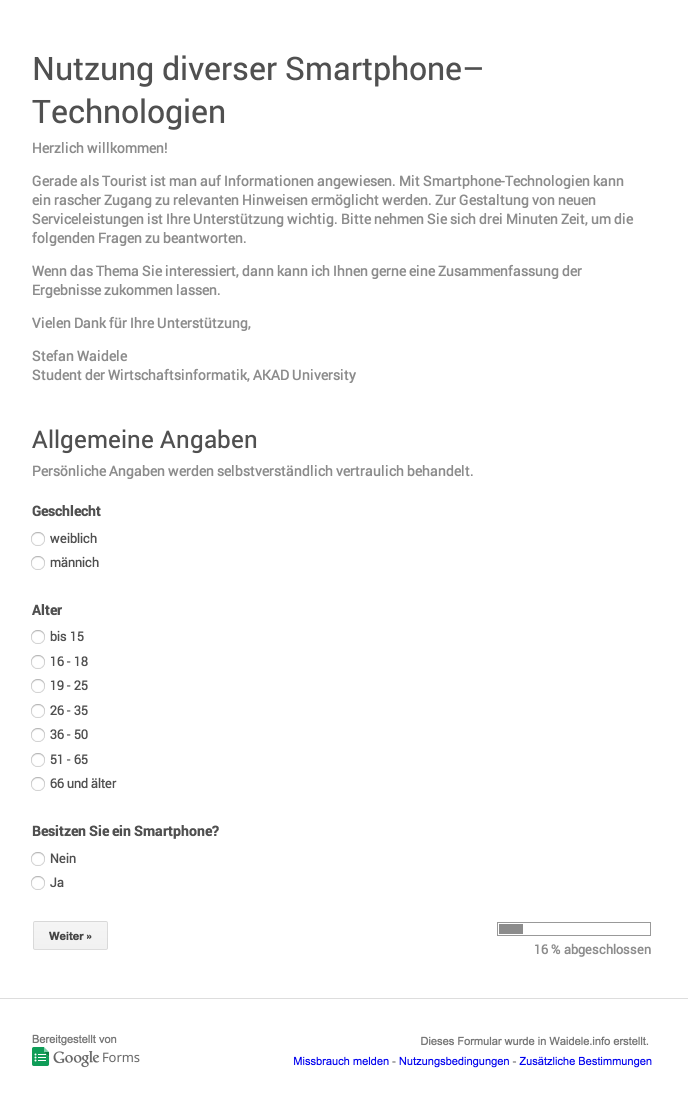
\includegraphics[width=.6\textwidth]{Umfrage-S1.png}
\caption{Screenshot: Umfrage Seite 1}
\label{pic:us1}
\end{center}
\end{figure}

\begin{figure}[H]
\begin{center}
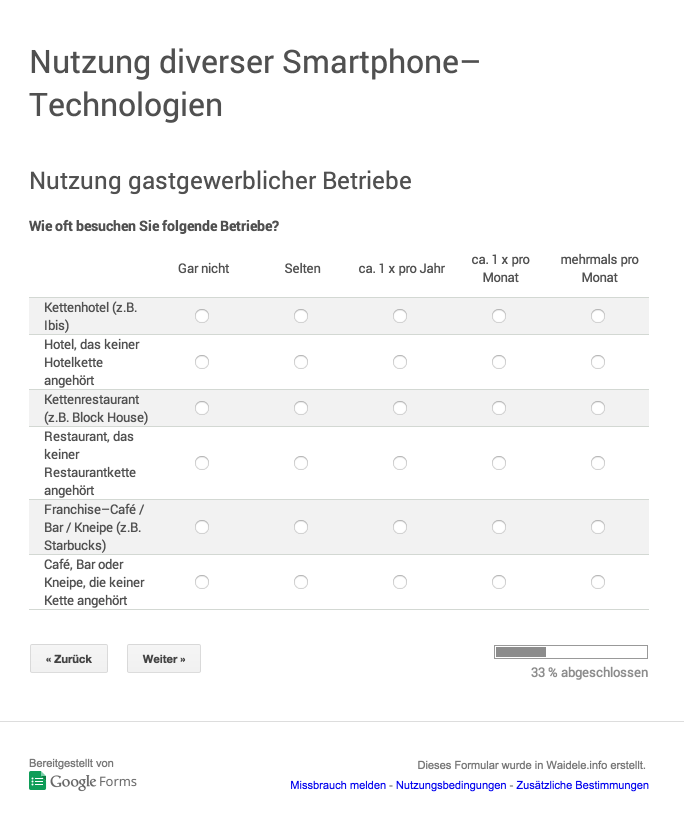
\includegraphics[width=.5\textwidth]{Umfrage-S2.png}
\caption{Screenshot: Umfrage Seite 2}
\label{pic:us2}
\end{center}
\end{figure}

\begin{figure}[H]
\begin{center}
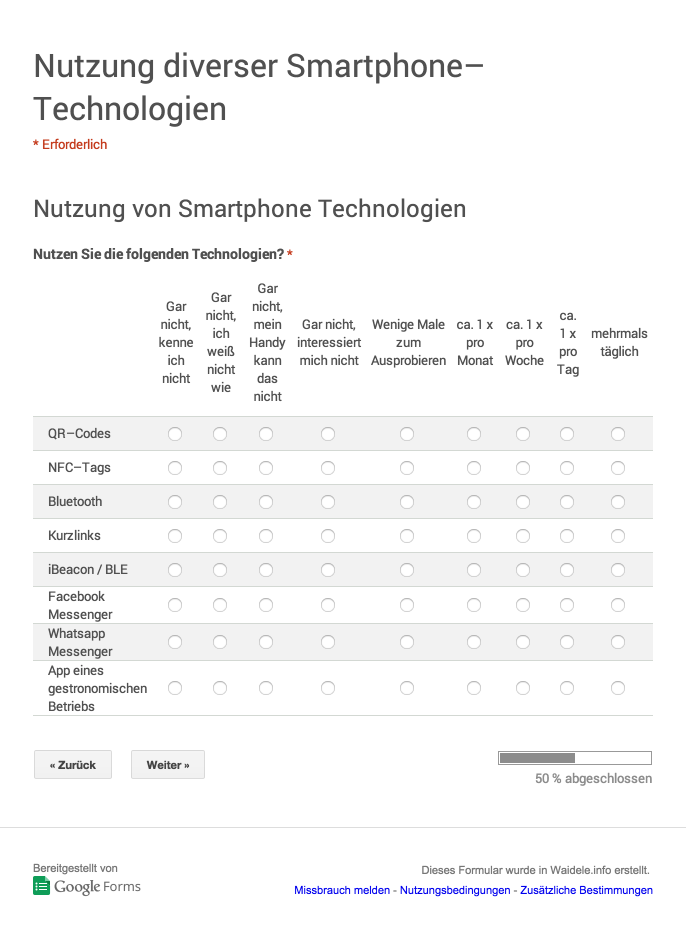
\includegraphics[width=.5\textwidth]{Umfrage-S3.png}
\caption{Screenshot: Umfrage Seite 3}
\label{pic:us3}
\end{center}
\end{figure}

\begin{figure}[H]
\begin{center}
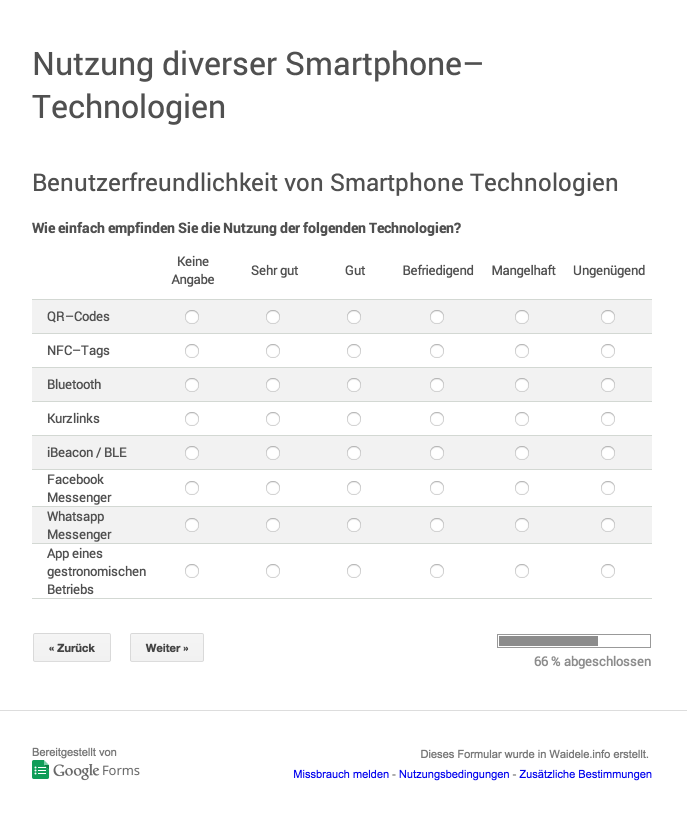
\includegraphics[width=.6\textwidth]{Umfrage-S4.png}
\caption{Screenshot: Umfrage Seite 4}
\label{pic:us4}
\end{center}
\end{figure}

\begin{figure}[H]
\begin{center}
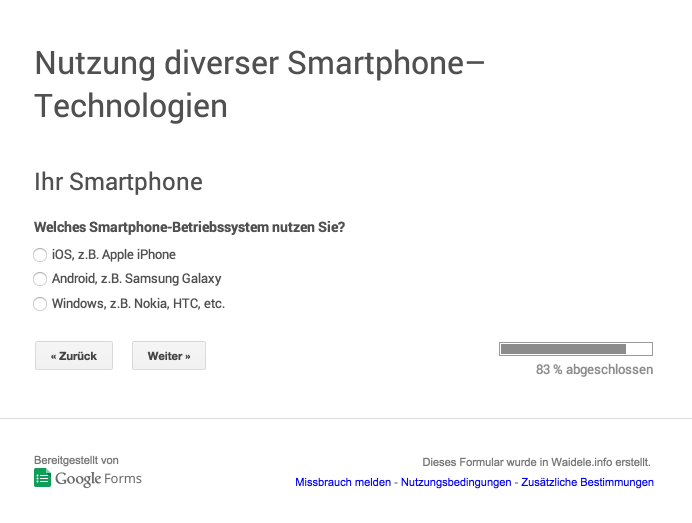
\includegraphics[width=.6\textwidth]{Umfrage-S5.png}
\caption{Screenshot: Umfrage Seite 5}
\label{pic:us5}
\end{center}
\end{figure}

\begin{figure}[H]
\begin{center}
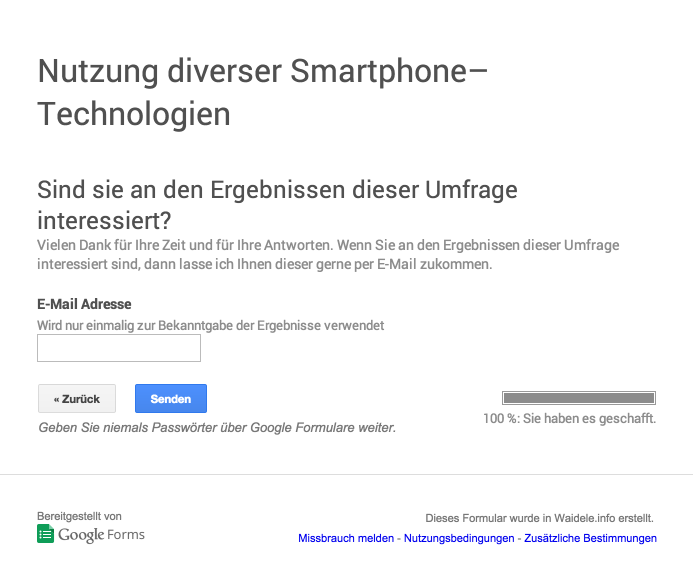
\includegraphics[width=.6\textwidth]{Umfrage-S6.png}
\caption{Screenshot: Umfrage Seite 6}
\label{pic:us6}
\end{center}
\end{figure}

\newpage
\subsection*{Anhang 2: Auswertung des Kundenfragebogens}
\addcontentsline{toc}{subsection}{Anhang 2: Auswertung des Kundenfragebogens}

Zwischen 12. August 2014 und 12. November 2014 wurden 174 Fragebögen ausgefüllt. 

Die Ergebnisse sind auf den Seiten \pageref{tab:geschlecht} bis \pageref{tab:usability} zusammengefasst. Differenzen zu 100\% entstehen durch Rundungsdifferenzen.

\begin{table}[H]
\begin{center}
\begin{footnotesize}
\begin{tabular}{| l | r  r |}  \hline                       
  \textbf{Geschlecht}              & \multicolumn{2}{|l|}{\textbf{Anzahl}}   \\ \hline 
  weiblich        &  109 &   (63\%)  \\  \hline  
  männlich        &  64  &   (37\%)  \\  \hline  
  keine Angabe    &  1   &   (<1\%)  \\  \hline  
  \textbf{Summe}  & 174  &   \\  \hline  
\end{tabular}
\end{footnotesize}
\caption{Auswertung: Geschlecht}
\label{tab:geschlecht}
\end{center}
\end{table}

\begin{table}[H]
\begin{center}
\begin{footnotesize}
\begin{tabular}{| l | r  r |}  \hline                       
  \textbf{Altersklasse}              & \multicolumn{2}{|l|}{\textbf{Anzahl}}   \\ \hline 
  bis 15          &  0 &   (0\%)  \\  \hline  
  16 bis 18       &  1 &   (<1\%)  \\  \hline  
  19 bis 25       & 20  &   (11\%)  \\  \hline  
  26 bis 35       & 95  &   (55\%)  \\  \hline  
  36 bis 50       & 42  &   (24\%)  \\  \hline  
  51 bis 65       & 16  &   (9\%)  \\  \hline  
  66 und älter    & 0  &   (0\%)  \\  \hline  
  \textbf{Summe}  & 174  &   \\  \hline  
\end{tabular}
\end{footnotesize}
\caption{Auswertung: Altersklassen}
\label{tab:altersklassen}
\end{center}
\end{table}

\begin{table}[H]
\begin{center}
\begin{footnotesize}
\begin{tabular}{| l | r  r |}  \hline                       
  \textbf{Smartphone}              & \multicolumn{2}{|l|}{\textbf{Anzahl}}   \\ \hline 
  ja        &  161 &   (93\%)  \\  \hline  
  nein        &  12  &   (7\%)  \\  \hline  
  keine Angabe    &  1   &   (<1\%)  \\  \hline  
  \textbf{Summe}  & 174  &   \\  \hline  
\end{tabular}
\end{footnotesize}
\caption{Auswertung: Smartphone}
\label{tab:smartphone}
\end{center}
\end{table}

\begin{table}[H]
\begin{center}
\begin{footnotesize}
\begin{tabular}{| l | r  r |}  \hline                       
  \textbf{Smartphone}              & \multicolumn{2}{|l|}{\textbf{Anzahl}}   \\ \hline 
  Android    &  83 &   (50\%)  \\  \hline  
  iOS        &  71  &   (43\%)  \\  \hline  
  Windows    &  12   &   (7\%)  \\  \hline  
  \textbf{Summe}  & 166  &   \\  \hline  
\end{tabular}
\end{footnotesize}
\caption{Auswertung: Betriebssysteme}
\label{tab:os}
\end{center}
\end{table}

\begin{table}[H]
\begin{center}
\begin{footnotesize}
\begin{tabular}{| l | C{1cm} | C{1cm} | C{1cm} | C{1cm} | C{1cm} |}  \hline
  \textbf{Frequenz} & 
	\begin{turn}{90}\textbf{Gar nicht}\end{turn} & 
	\begin{turn}{90}\textbf{Selten}\end{turn}  & 
	\begin{turn}{90}\textbf{ca. 1 x pro Jahr}\end{turn} & 
	\begin{turn}{90}\textbf{ca. 1 x pro Monat}\end{turn} & 
	\begin{turn}{90}\textbf{mehrmals monatlich}\end{turn}\\ \hline 
	\multirow{2}{*}{Kettenhotel}  & 27 & 59 & 59 & 23 & 6\\  
		                          & (16\%) & (34\%) & (34\%) & (13\%) & (3\%) \\  \hline  
	\multirow{2}{*}{Individualhotel} & 13 & 67 & 76 & 16 & 2\\   
		                             & (7\%) & (39\%) & (44\%) & (9\%) & (1\%) \\  \hline  
	\multirow{2}{*}{Kettenrestaurant} 	 & 26 & 48  & 57  & 38   & 5\\  
		      & (15\%) & (28\%) & (33\%) & (22\%) & (3\%) \\  \hline  
	\multirow{2}{*}{Individualrestaurant} &  8  & 20   & 30  & 86   & 30\\   
		      & (5\%) & (11\%) & (17\%) & (49\%) & (17\%) \\  \hline  
	\multirow{2}{*}{Kettencafé} &  24  &  55  & 38  & 42   & 15\\  
		      & (14\%) & (32\%) & (22\%) & (24\%) & (7\%) \\  \hline  
	\multirow{2}{*}{Individualcafé} & 7   &  24  & 18  & 77   & 48\\   
		      & (4\%) & (14\%) & (10\%) & (44\%) & (28\%) \\  \hline  
\end{tabular}
\end{footnotesize}
\caption{Auswertung: Nutzung gastgewerblicher Betriebe}
\label{tab:gastronutzung}
\end{center}
\end{table}


\begin{table}[H]
\begin{center}
\begin{footnotesize}
\begin{tabular}{| l | C{1cm} | C{1cm} | C{1cm} | C{1cm} | C{1cm} | C{1cm} | C{1cm} | C{1cm} | C{1cm} |}  \hline
  \textbf{Technologie} & 
	\begin{turn}{90}\textbf{Gar nicht, …}\end{turn} & 
	\begin{turn}{90}\textbf{Wenige male zum Ausprobieren}\end{turn}  & 
	\begin{turn}{90}\textbf{ca. 1 x pro Monat}\end{turn} & 
	\begin{turn}{90}\textbf{ca. 1 x pro Woche}\end{turn} & 
	\begin{turn}{90}\textbf{ca. 1 x am Tag}\end{turn} & 
	\begin{turn}{90}\textbf{mehrmals täglich}\end{turn}\\ \hline 
	\multirow{2}{*}{QR Codes}   &  62    &  82    &  22    &  8   &  \multirow{2}{*}{—}    & \multirow{2}{*}{—}    \\  
		                       & (36\%) & (47\%) & (13\%) & (5\%) &  &  \\  \hline  
	\multirow{2}{*}{NFC Tags}   &  142    &  26    &  4    &  2   &  \multirow{2}{*}{—}    & \multirow{2}{*}{—}    \\  
		                       & (82\%) & (15\%) & (2\%) & (1\%) &  &  \\  \hline  
	\multirow{2}{*}{Bluetooth}    &  34    & 35     & 37     & 23    & 17     & 28    \\  
		                       & (20\%)    & (20\%) & (21\%) & (13\%) & (10\%) & (16\%) \\  \hline  
	\multirow{2}{*}{iBeacon / BLE}    & 161     & 11     &   \multirow{2}{*}{—}    &  \multirow{2}{*}{—}    &  2    &  \multirow{2}{*}{—}    \\  
		                              & (93\%) & (6\%) &  &  & (1\%) &  \\  \hline  
	\multirow{2}{*}{Kurzlinks}    & 70     &  23    & 29     & 21    &  12    & 19    \\  
		                          & (40\%) & (13\%) & (17\%) & (12\%) & (7\%) & (11\%) \\  \hline  
	\multirow{2}{*}{Facebook Messenger}    &  78    &  11    & 8     & 17    & 21     & 39    \\  
		                                   & (45\%) & (6\%) & (5\%) & (10\%) & (12\%) & (22\%) \\  \hline  
	\multirow{2}{*}{Whatsapp Messenger}    & 32     & 1     & 2     & 14    &  18    & 107    \\  
		                                   & (18\%) & (<1\%) & (1\%) & (8\%) & (10\%) & (61\%) \\  \hline  
	\multirow{2}{*}{App eines Betriebes}   & 98     & 45     & 23     & 5    &  2    & 1    \\  
		                                   & (56\%) & (26\%) & (13\%) & (3\%) & (1\%) & (<1\%) \\  \hline  
\end{tabular}
\end{footnotesize}
\caption{Auswertung: Nutzung von Smartphone Technologien}
\label{tab:technutzung}
\end{center}
\end{table}

\begin{table}[H]
\begin{center}
\begin{footnotesize}
\begin{tabular}{| l | C{1cm} | C{1cm} | C{1cm} | C{1cm} |}  \hline
  \textbf{Technologie} & 
  	\begin{turn}{90}\textbf{Gar nicht, interessiert mich nicht}\end{turn} &
	\begin{turn}{90}\textbf{Gar nicht, kenne ich nicht}\end{turn} & 
	\begin{turn}{90}\textbf{Gar nicht, ich weiß nicht wie}\end{turn} & 
	\begin{turn}{90}\textbf{Gar nicht, mein Handy kann das nicht}\end{turn} \\ \hline 
	\multirow{2}{*}{QR Codes}  &  28    & 26     & 2     & 6     \\  
		                       & (16\%) & (15\%) & (1\%) & (3\%) \\  \hline  
	\multirow{2}{*}{NFC Tags}  &  38    & 72     & 5     &  27    \\  
		                       & (22\%) & (41\%) & (3\%) & (16\%) \\  \hline  
	\multirow{2}{*}{Bluetooth}  &  22    & 7     & 2     & 3     \\  
		                       & (13\%) & (4\%) & (1\%) & (2\%) \\  \hline  
	\multirow{2}{*}{iBeacon / BLE}   &  28    & 117     & 6     & 10     \\  
		                       & (16\%) & (67\%) & (3\%) & (6\%) \\  \hline  
	\multirow{2}{*}{Kurzlinks}   & 28     & 35     & 2     & 5     \\  
		                         & (16\%) & (20\%) & (1\%) & (3\%) \\  \hline  
	\multirow{2}{*}{Facebook Messenger}   & 59     & 9     & 2     & 8     \\  
		                                  & (34\%) & (5\%) & (1\%) & (5\%) \\  \hline  
	\multirow{2}{*}{Whatsapp Messenger}   & 19     & 4     &  \multirow{2}{*}{—}    &  9    \\  
		                                  & (11\%) & (2\%) &  & (5\%) \\  \hline  
	\multirow{2}{*}{App eines Betriebes}  & 59     & 26     & 4     & 9     \\  
		                                  & (34\%) & (15\%) & (2\%) & (5\%) \\  \hline  
\end{tabular}
\end{footnotesize}
\caption{Auswertung: Gründe für die Nicht–Nutzung}
\label{tab:nichtnutzung}
\end{center}
\end{table}

\begin{table}[H]
\begin{center}
\begin{footnotesize}
\begin{tabular}{| l | C{1cm} | C{1cm} | C{1cm} | C{1cm} | C{1cm} | C{1cm} | C{1cm} | C{1cm} | C{1cm} |}  \hline
  \textbf{Technologie} & 
	\begin{turn}{90}\textbf{Keine Angabe}\end{turn} & 
	\begin{turn}{90}\textbf{Sehr gut}\end{turn}  & 
	\begin{turn}{90}\textbf{Gut}\end{turn} & 
	\begin{turn}{90}\textbf{Befriedigend}\end{turn} & 
	\begin{turn}{90}\textbf{Mangelhaft}\end{turn} & 
	\begin{turn}{90}\textbf{Ausreichend}\end{turn}\\ \hline 
	\multirow{2}{*}{QR Codes}   & 57     & 41     & 50     & 21    &  2    & 3    \\  
		                        & (33\%) & (24\%) & (29\%) & (12\%) & (1\%) & (2\%) \\  \hline  
	\multirow{2}{*}{NFC Tags}   & 130    & 10    & 17     & 12    & 4     & 1    \\  
		                        & (75\%) & (6\%) & (10\%) & (7\%) & (2\%) & (<1\%) \\  \hline  
	\multirow{2}{*}{Bluetooth}  & 24     & 56     & 63     & 25    & 5     & 1    \\  
		                        & (14\%) & (32\%) & (36\%) & (14\%) & (3\%) & (<1\%) \\  \hline  
	\multirow{2}{*}{iBeacon / BLE} & 160    & 1     & 4     & 4    & 2     & 3    \\  
		                           & (92\%) & (<1\%) & (2\%) & (2\%) & (1\%) & (2\%) \\  \hline  
	\multirow{2}{*}{Kurzlinks}  &  61    & 45     & 52     & 8    & 6     & 2    \\  
		                        & (35\%) & (26\%) & (30\%) & (5\%) & (3\%) & (1\%) \\  \hline  
	\multirow{2}{*}{Facebook Messenger} & 60     & 26     & 45     & 26    & 6     & 11    \\  
		                                & (34\%) & (15\%) & (26\%) & (15\%) & (3\%) & (6\%) \\  \hline  
	\multirow{2}{*}{Whatsapp Messenger} & 32     & 76     & 52     & 5    & 6     & 3    \\  
		                                & (18\%) & (44\%) & (30\%) & (3\%) & (3\%) & (2\%) \\  \hline  
	\multirow{2}{*}{App eines Betriebes}  & 113    & 4     & 29     & 19    & 8     & 1    \\  
		                                  & (65\%) & (2\%) & (17\%) & (11\%) & (5\%) & (<1\%) \\  \hline  
\end{tabular}
\end{footnotesize}
\caption{Auswertung: Benutzerfreundlichkeit von Smartphone Technologien}
\label{tab:usability}
\end{center}
\end{table}


\end{spacing}

\clearpage

% Literaturverzeichniss - Ab hier wieder Roemische Seitenzahlen
\pagestyle{plain}
\pagenumbering{roman}
\setcounter{page}{\theromanPagenumber}
%\addcontentsline{toc}{section}{Literatur-- und Quellenverzeichnis}
\renewcommand{\refname}{Literatur-- und Quellenverzeichnis}
\bibliographystyle{alpha}
\bibliography{pb-literatur}
\onehalfspacing
\clearpage

\pagestyle{empty} 
\thispagestyle{empty}

\begin{center}
{\Large Eidesstattliche Erklärung}
\vspace*{4cm}\end{center}
\noindent
Ich versichere, dass ich das beiliegende Assignment selbstständig verfasst, keine anderen als die angegebenen Quellen und Hilfsmittel benutzt sowie alle wörtlich oder sinngemäß übernommenen Stellen in der Arbeit gekennzeichnet habe. 
\vspace{3cm}

\hspace{-0.8cm}
\rule[0.5ex]{6.5cm}{1pt}
\hspace{1.3cm}
\rule[0.5ex]{6.5cm}{1pt}
\\(Datum, Ort)
\hspace{6.3cm}
(Unterschrift)


\end{document}

